\documentclass[15pt,a4paper]{report}
%
% This LaTeX template has been created by Luca Grilli
% Based on the following https://en.wikibooks.org/wiki/LaTeX/Title_Creation
% 
\usepackage[italian]{babel}
%\usepackage[T1]{fontenc} % Riga da commentare se si compila con PDFLaTeX
\usepackage{geometry}
\usepackage{graphicx}
\usepackage{hyperref}
\usepackage[utf8]{inputenc}
\usepackage{lipsum} % genera testo fittizio
\usepackage{subcaption}
\usepackage[nottoc,numbib]{tocbibind}
\usepackage{titlesec}
\usepackage{crimson}
\usepackage[simplified]{pgf-umlcd}
\usepackage{float}
\usepackage{wrapfig,lipsum}
\usepackage{fancyhdr, etoolbox}
\usepackage{listings}
\usepackage{xcolor}
\usepackage{url}
\usepackage{setspace}
\usepackage{longtable}
\include{json-lang}

% Copyright 2017 Sergei Tikhomirov, MIT License
% https://github.com/s-tikhomirov/solidity-latex-highlighting/

\usepackage{listings, xcolor}

\definecolor{verylightgray}{rgb}{.97,.97,.97}

\lstdefinelanguage{Solidity}{
	keywords=[1]{anonymous, assembly, assert, balance, break, call, callcode, case, catch, class, constant, continue, constructor, contract, debugger, default, delegatecall, delete, do, else, emit, event, experimental, export, external, false, finally, for, function, gas, if, implements, import, in, indexed, instanceof, interface, internal, is, length, library, log0, log1, log2, log3, log4, memory, modifier, new, payable, pragma, private, protected, public, pure, push, require, return, returns, revert, selfdestruct, send, solidity, storage, struct, suicide, super, switch, then, this, throw, transfer, true, try, typeof, using, value, view, while, with, addmod, ecrecover, keccak256, mulmod, ripemd160, sha256, sha3}, % generic keywords including crypto operations
	keywordstyle=[1]\color{blue}\bfseries,
	keywords=[2]{address, bool, byte, bytes, bytes1, bytes2, bytes3, bytes4, bytes5, bytes6, bytes7, bytes8, bytes9, bytes10, bytes11, bytes12, bytes13, bytes14, bytes15, bytes16, bytes17, bytes18, bytes19, bytes20, bytes21, bytes22, bytes23, bytes24, bytes25, bytes26, bytes27, bytes28, bytes29, bytes30, bytes31, bytes32, enum, int, int8, int16, int24, int32, int40, int48, int56, int64, int72, int80, int88, int96, int104, int112, int120, int128, int136, int144, int152, int160, int168, int176, int184, int192, int200, int208, int216, int224, int232, int240, int248, int256, mapping, string, uint, uint8, uint16, uint24, uint32, uint40, uint48, uint56, uint64, uint72, uint80, uint88, uint96, uint104, uint112, uint120, uint128, uint136, uint144, uint152, uint160, uint168, uint176, uint184, uint192, uint200, uint208, uint216, uint224, uint232, uint240, uint248, uint256, var, void, ether, finney, szabo, wei, days, hours, minutes, seconds, weeks, years},	% types; money and time units
	keywordstyle=[2]\color{teal}\bfseries,
	keywords=[3]{block, blockhash, coinbase, difficulty, gaslimit, number, timestamp, msg, data, gas, sender, sig, value, now, tx, gasprice, origin},	% environment variables
	keywordstyle=[3]\color{violet}\bfseries,
	identifierstyle=\color{black},
	sensitive=false,
	comment=[l]{//},
	morecomment=[s]{/*}{*/},
	commentstyle=\color{gray}\ttfamily,
	stringstyle=\color{red}\ttfamily,
	morestring=[b]',
	morestring=[b]"
}

\lstset{
	language=Solidity,
	backgroundcolor=\color{verylightgray},
	extendedchars=true,
	basicstyle=\footnotesize\ttfamily,
	showstringspaces=false,
	showspaces=false,
	numbers=left,
	numberstyle=\footnotesize,
	numbersep=9pt,
	tabsize=2,
	breaklines=true,
	showtabs=false,
	captionpos=b
}


\usetikzlibrary{calc} 
\pagestyle{fancy}

\fancyhead{}
\fancyhead[OL]{\ifnumodd{\value{page}}{\slshape \leftmark}{\slshape SEZIONE \rightmark}}
\fancypagestyle{mystyle}{
    \fancyhead[OL]{\slshape \leftmark}
}
\fancyfoot[C]{\thepage}

\fontfamily{bch}\selectfont

% Taken from Lena Herrmann at 
% http://lenaherrmann.net/2010/05/20/javascript-syntax-highlighting-in-the-latex-listings-package

\usepackage{color} %use color
\definecolor{mygreen}{rgb}{0,0.6,0}
\definecolor{mygray}{rgb}{0.5,0.5,0.5}
\definecolor{mymauve}{rgb}{0.58,0,0.82}

%Customize a bit the look
\lstset{ %
backgroundcolor=\color{white}, % choose the background color; you must add \usepackage{color} or \usepackage{xcolor}
basicstyle=\footnotesize, % the size of the fonts that are used for the code
breakatwhitespace=false, % sets if automatic breaks should only happen at whitespace
breaklines=true, % sets automatic line breaking
captionpos=b, % sets the caption-position to bottom
commentstyle=\color{mygreen}, % comment style
deletekeywords={...}, % if you want to delete keywords from the given language
escapeinside={<@}{@>}, % if you want to add LaTeX within your code
extendedchars=true, % lets you use non-ASCII characters; for 8-bits encodings only, does not work with UTF-8
frame=single, % adds a frame around the code
keepspaces=true, % keeps spaces in text, useful for keeping indentation of code (possibly needs columns=flexible)
keywordstyle=\color{blue}, % keyword style
% language=Octave, % the language of the code
morekeywords={*,...}, % if you want to add more keywords to the set
numbers=left, % where to put the line-numbers; possible values are (none, left, right)
numbersep=5pt, % how far the line-numbers are from the code
numberstyle=\tiny\color{mygray}, % the style that is used for the line-numbers
rulecolor=\color{black}, % if not set, the frame-color may be changed on line-breaks within not-black text (e.g. comments (green here))
showspaces=false, % show spaces everywhere adding particular underscores; it overrides 'showstringspaces'
showstringspaces=false, % underline spaces within strings only
showtabs=false, % show tabs within strings adding particular underscores
stepnumber=1, % the step between two line-numbers. If it's 1, each line will be numbered
stringstyle=\color{mymauve}, % string literal style
tabsize=2, % sets default tabsize to 2 spaces
title=\lstname, % show the filename of files included with \lstinputlisting; also try caption instead of title
}
%END of listing package%

\definecolor{darkgray}{rgb}{.4,.4,.4}
\definecolor{purple}{rgb}{0.65, 0.12, 0.82}

%define Javascript language
\lstdefinelanguage{JavaScript}{
keywords={typeof, new, true, false, catch, function, return, null, catch, switch, var, if, while, do, else, case, break, for, of, const, async, await},
keywordstyle=\color{blue}\bfseries,
ndkeywords={class, export, boolean, throw, implements, import},
ndkeywordstyle=\color{darkgray}\bfseries,
identifierstyle=\color{black},
sensitive=false,
comment=[l]{//},
morecomment=[s]{/*}{*/},
commentstyle=\color{purple}\ttfamily,
stringstyle=\color{red}\ttfamily,
morestring=[b]',
morestring=[b]"
}

\lstset{
language=JavaScript,
extendedchars=true,
basicstyle=\footnotesize\ttfamily,
showstringspaces=false,
showspaces=false,
numbers=left,
numberstyle=\footnotesize,
numbersep=9pt,
tabsize=2,
breaklines=true,
showtabs=false,
captionpos=b
}


\titleformat{\chapter}[display]{\Huge\bfseries}{}{0pt}{\thechapter.\ }

\graphicspath{{figures/}}
%
%\addtolength{\topmargin}{-.875in} % reduce the default top margin
%\addtolength{\topmargin}{-2cm} % reduce the default top margin
%

\tolerance=1
\emergencystretch=\maxdimen
\hyphenpenalty=10000
\hbadness=10000

%%%%%%%%%%%%%%%%%%%%%%%%%%%%%%%%%%
%                                %
%     Begin Docuemnt [start]     %
%                                %
%%%%%%%%%%%%%%%%%%%%%%%%%%%%%%%%%%
\begin{document}

\begin{titlepage}

%%%%%%%%%%%%%%%%%%%%%%%%%%%%%%
%     Title Page [start]     %
%%%%%%%%%%%%%%%%%%%%%%%%%%%%%%
% Declare new goemetry for the title page only.
{\Large \noindent Francesca Nocentini} \newline

\vspace{1cm}

{\begin{flushleft}
\fontsize{21.8}{26.16} \selectfont \bfseries \noindent 
Tecniche di deep learning \\
per la classificazione \\
di immagini biomedicali
\end{flushleft}}

\vspace{6mm}

{\large \noindent \emph{Relatore}: \vspace{1.0mm}\\ 
Prof. Gianluca Reali \newline}

\vspace{5cm}


\noindent Perugia, Anno Accademico 2020/2021 

\noindent Università degli Studi di Perugia \\
Corso di laurea triennale in Ingegneria Informatica ed Elettronica \\
Dipartimento di Ingegneria

\vspace{0.7cm}

\noindent 
\includegraphics[width=0.5\textwidth]{figures/logounipg2021.png}
% Ends the declared geometry for the titlepage
\restoregeometry
\end{titlepage}
\normalfont
%%%%%%%%%%%%%%%%%%%%%%%%%%%%
%     Title Page [end]     %
%%%%%%%%%%%%%%%%%%%%%%%%%%%%
\newpage \thispagestyle{empty} \ \newpage
%%%%%%%%%%%%%%%%%%%%%%%%%%
%     Indice [start]     %
%%%%%%%%%%%%%%%%%%%%%%%%%%
\onehalfspacing
\tableofcontents

%%%%%%%%%%%%%%%%%%%%%%%%
%     Indice [end]     %
%%%%%%%%%%%%%%%%%%%%%%%%

 
\chapter{Introduzione}

Al giorno d’oggi, con l’avvento delle tecnologie di imaging biomedico,
 il numero di immagini che sono state catturate ed archiviate giorno dopo giorno negli ospedali 
 e nei laboratori sta crescendo sempre di più. Con questo però, di pari passo all'avanzamento tecnologico, che preveda sistemi  
  più robusti e all’avanguardia affinchè vengano raggiunti gli obiettivi di diagnosi e classificazione di 
  vari tipi di patologie. 
Sulla scia di ciò, per assistere medici e specialisti, queste immagini possono essere usate 
ed utilizzate per allenare sistemi intelligenti. Pertanto in virtù di questa grande quantità di 
immagini mediche (ecografie, mammografie, MRI...), l’uso di metodi basate sulle \emph{big data technologies}, 
come il machine learning (ML) e l’Intelligenza Artificiale è diventato fondamentale, 
anche e soprattutto come supporto all’equipe medica. 
Sono stati dunque proposti negli anni dei metodi per automatizzare il processo di analisi
 di immagine medica. 
Nel presente lavoro di tesi saranno analizzati ed utilizzati metodi di classificazione di 
immagini usando metodi di deep learning. Questi ultimi non sono altro che un’evoluzione dei metodi di ML 
atti a trattare dati di grande cardinalità e complessità. \\
In particolare  in una prima parte verrà
 fatta una discriminazione tra soggetti affetti da polmonite e soggetti sani tramite l’utilizzo
  di radiografie al petto; in una seconda parte invece il sistema viene allenato in modo tale da 
  poter classificare immagini di risonanze magnetiche cerebrali tra 4 diverse diagnosi per 
  il soggetto nell’immagine: glioma, meningioma, tumore ipofisario e soggetto sano.




\chapter{Machine learning e le reti neurali}

\section{L'importanza dell'apprendimento}

Le reti neurali sono alla base del deep learning, che è un sottocampo del machine learning.
Questa ultima branca è fondamentale nello studio e nello sviluppo delle Intelligenze Artificiali, sistemi basati sull’apprendimento automatico partendo dallo studiare i dati in input per fornire dati più vicini possibile a quelli desiderati. 
Sostanzialmente un algoritmo di machine learning è un algoritmo capace di apprendere dai dati. \\

\emph{"Si dice che un programma apprende dall'esperienza E con riferimento a alcune classi di
 compiti T e con misurazione della performance P, se le sue performance nel compito T, come misurato da P,
  migliorano con l'esperienza E." } 

Tom M. Mitchell\footnote{Tom Michael Mitchell è un computer scientist americano e professore universitario. É conosciuto per aver contribuito attivamente allo sviluppo degli studi sul machine learining e le intelligenze artificiali.} \\

Il compito principale del machine learning è che una macchina sia in grado di generalizzare
 dalla propria esperienza. Per generalizzazione si intende l'abilità di una macchina di portare a
  termine in maniera accurata esempi o compiti nuovi, che non ha mai affrontato, 
  dopo aver fatto esperienza su un insieme di dati di apprendimento.\\
La macchina ha il compito di costruire un modello probabilistico generale dello spazio delle 
occorrenze di un determinato fenomeno da apprendere tramite dei \emph{training examples}, in maniera 
tale da essere in grado di produrre previsioni sufficientemente accurate quando sottoposta a nuovi casi. 
Proprio a questo proposito, al fine di valutare la bontà di un algoritmo di machine learning,
 dobbiamo stimare un andamento qualitativo della sua performance P, la quale molto spesso è specifica 
 per un determinato compito T che il sistema deve compiere. 

I compiti dell'apprendimento automatico vengono tipicamente classificati in tre ampie categorie, 
sulla base dell’esperienza E a cui sono sottoposti nel processo di apprendimento, dunque a seconda 
della natura del "segnale" utilizzato per l'apprendimento o del "feedback" disponibile al sistema di
 apprendimento. Queste categorie, anche dette paradigmi, sono:
 \begin{itemize}
\item \textbf{apprendimento supervisionato}, in cui al modello vengono forniti degli esempi nella forma
 di possibili input e output desiderati e l'obiettivo è quello di estrarre una regola
  generale che associ l'input all'output corretto;
\item \textbf{apprendimento non supervisionato}, in cui il modello ha lo scopo di trovare una
 struttura negli 
input forniti, senza che gli input vengano etichettati in alcun modo;
\item apprendimento per rinforzo, il quale punta a realizzare agenti 
autonomi in grado di scegliere
 azioni da compiere per il conseguimento di determinati obiettivi tramite interazione con l'ambiente
  in cui sono immersi. 
\end{itemize}
Il tipo di apprendimento di interesse per il lavoro di tesi è quello supervisionato, in quanto si utilizzano coppie input-output 
rappresentate da immagini e label che le identificano. \\
Tra i compiti più importanti dell’apprendimento supervisionato vi sono la classificazione
 e la regressione, i quali si distinguono a seconda di come viene considerato l’output 
 del sistema di apprendimento. 
 Nella prima gli output sono divisi in due o più classi e il sistema di apprendimento 
 deve produrre un modello che assegni gli input non ancora visti a una o più di queste. 
 Si dice che i valori assunti dall'ouput sono \emph{qualitativi}. 
 Nella seconda invece si può dire che a differenza della prima i dati in output sono continui, 
 cioè non riguardano una categorizzazione. Si dice i valori assunti dall'output sono \emph{quantitativi},
  in quanto restituiscono la stima di una misura. \\
La classificazione è il compito su cui verte il presente lavoro di tesi.
 Per tale scopo, la performance P dell’algoritmo di machine learning si valuta misurando
  l’accuratezza del modello, la percentuale di esempi per i quali il modello elabora un output 
  corretto sul totale delle osservazioni. Un altro parametro di riferimento può essere il rate di errore,
   definito invece come la
    proporzione di esempi per cui il sistema elabora un output sbagliato.
E’ importante verificare come l’algoritmo riesca a valutare dati che non abbia mai visto.
 Misure di performance vengono effettuate usando un insieme di dati chiamato insieme di \emph{test}.
  Questo insieme di dati è, di solito, diverso dall’insieme di caratteristiche usate per allenare 
  il sistema (insieme di \emph{addestramento} o \emph{training}) affinchè si possano fare valutazioni
   più precise ed indipendenti su quanto sia stato efficace l’addestramento.
Di solito l’esperienza E corrisponde ad un intero \emph{dataset}, una collezione di dati
 (che possono essere sotto forma di vettori, immagini, suoni ecc.) 
 suddiviso in classi con ogni elemento associato ad una ed una sola di queste. Tali dati, essendo utilizzati
  in fase di addestramento, è estremamente importante che siano costruito in maniera corretta.
  Dunque il punto di partenza per un buon addestramento è sicuramente un buon dataset.
 \\
 
Come accennato sopra, l’apprendimento supervisionato è una forma di apprendimento automatico
 in cui al sistema da allenare si sottopone in input un insieme di addestramento formato da esempi
  etichettati con il rispettivo valore di output desiderato, e tra gli input e output si vuol trovare una corrispondenza.
   Questo processo fa tipicamente 
  riferimento a tecniche
  di tipo statistico.
Esso consiste nell’osservazione di una quantità di esempi di un vettore casuale 
\textbf{x} a cui è associato un vettore \textbf{y}  per poi apprendere come predire \textbf{y} 
da \textbf{x}, 
stimando una distribuzione
 di probabilità condizionata p(\textbf{y}$\mid$\textbf{x})\footnote{Date due variabili aleatorie X e Y,
  la distribuzione condizionata di Y dato X è la probabilità di Y quando è conosciuto il valore 
  assunto da X} per l'output, che consenta di ottenere anche valori di 
 confidenza per l'algoritmo. I valori di \textbf{y} fungono da guida per indirizzare e migliorare 
 l’apprendimento di contro al caso non supervisionato in cui l’algoritmo deve trattare i dati 
 senza l’ausilio di questa guida. 
 Lo scopo degli algoritmi di machine learning è di derivare, a partire dal training set, una distribuzione
  di probabilità p(\textbf{y}$\mid$\textbf{x}) per l’output, che consenta ad esempio di ottenere
anche dei valori di confidenza. \\
Un esempio di apprendimento supervisionato è  il training di un sistema
col compito di riconoscimento delle immagini.
In questo caso dobbiamo specificare quale oggetto appare in ogni foto.
Possiamo fare questo con un codice numerico che caratterizzi le varie classi, per esempio
usando 0 per le persone, 1 per le macchine, 2 per i gatti, e così via, a seconda di quello che
 è il caso di interesse.\\


\section{Neuroni artificiali e deep learning}

Le \emph{reti neurali} si riferiscono storicamente alla rete di neuroni che si trovano nel cervello dei mammiferi,
 e la loro struttura ne ha ispirato gli algoritmi. I neuroni sono le unità fondamentali di calcolo, 
 e sono connessi tra loro in reti per processare dati. Essi rispondono a stimoli esterni, così come 
 le reti neurali prendono dati in input, si allenano nel riconoscere dei pattern ripetuti all’interno 
 dei dati, e sono in grado di predire l’output per un set di dati simili. La corteccia cerebrale umana
  contiene circa 1010 neuroni. Sono collegati tra loro da filamenti nervosi (assoni) che si diramano e
   terminano in sinapsi, connessioni verso altri neuroni. Le sinapsi connettono verso i dendriti, 
   diramazioni che si estendono dal corpo della cellula neurale e sono atti a ricevere impulsi da 
   altri neuroni nella forma di segnali elettrici. Nelle reti neurali biologiche lo spessore dei 
   dendriti definisce il peso ad esso associato. La rete risultante di neuroni tra loro connessi 
   nella corteccia cerebrale è responsabile del processare immagini, audio e dati sensoriali. 
   In presenza di una differenza di potenziale fra esterno e l’interno della cellula, il neurone 
   si attiva trasmettendo un impulso elettrico attraverso il suo assone che provoca la liberazione
    di un neurotrasmettitore.\\
Nelle reti neurali artificiali, il modo in cui le informazioni sono processate e i segnali 
sono trasferiti sono ampiamente idealizzati da tali concetti. 

 Il primo modello computazionale di neurone è stato proposto nel 1943 da Warren MuCulloch
  e Walter Pitts \footnote{McCulloch e Pitts sono un neurofisiologo e un logico americani}. 
McCulloch and Pitts hanno pensato ad un modello di neurone come un’unità di \emph{threshold} (soglia) binaria.
 Essa possiede due possibili stati: attivo o inattivo.\\
  Per ottenere il segnale di output il neurone elabora una 
 somma pesata degli input: se la somma eccede un certo valore di threshold, lo stato del neurone
  risulta attivo, altrimenti inattivo.
Il modello, in intervalli discreti di tempo t = 0, 1, 2, 3… , svolge del calcolo computazionale. \\
Lo stato del neurone numero j al passo t è identificato come:

\[s_j(t) = \left\{\begin{matrix}
    1 & \text{attivo}\\ 
    -1 & \text{non attivo}
    \end{matrix}\right.\]


Ricevuti in ingresso N stati \(s_j(t)\), il neurone numero i calcola 
\begin{equation} \label{1}
s_i(t+1)= sgn(\sum_{j=1}^{N}w_{ij}s_j(t)-\theta_i)= sgn(b_i(t))
\end{equation}

Infatti, dato un neurone avente N canali di ingresso \(s_1\), ···, \(s_N\) ad ognuno dei quali
è associato un peso \(w_ij\), il cui primo indice i si riferisce al neurone che fa il calcolo,
invece l’indice j rappresenta tutti 
i neuroni connessi al neurone i. Il valore del peso è rappresentato da un numero reale, 
che riproduce lo spessore e la conducibilità delle sinapsi neurali.
 Il segnale di uscita al passo \(t+1\) è ricavato attraverso la la somma pesata degli ingressi, 
detta livello di attivazione o \emph{local field} \(b_i(t)\). 
Alla somma pesata vediamo nella [1] essere sottratto il valore di threshold, denotato come \(\theta_i\). 
Nel campo del deep learning di cui si parlerà a breve esso è conosciuto 
anche come \emph{bias}, ed è necessario per la robustezza della rete neurale. Può essere identificato
 come un ulteriore canale di ingresso \(s_0\) che serve per alzare o 
abbassare la soglia di attivazione del neurone (threshold), dove per soglia indichiamo il livello oltre
 al quale il neurone risulta attivo. 
La somma pesata e shiftata viene poi passata per una determinata funzione f, 
che nel caso del neurone di McCulloch e Pitts  è la funzione segno \emph{sgn()}.
Nel deep learning la funzione segno è molto spesso sostituita da una funzione f chiamata
 \emph{funzione di attivazione}. La funzione di attivazione definisce l’uscita di un neurone 
 in funzione del suo livello di attivazione \(b_i(t)\).
Una scelta comunemente utilizzata è la sigmoide: 
\[f(x)= \frac{1}{1+\mathrm{e}^{-x}}\]
Un’altra molto importante e anch’essa utilizzata è la ReLU (Rectified Linear Unit):
\[f(x) = x^{+} = max(0,x)\]

Tale funzione è una delle più utilizzate negli algoritmi di deep learning per la rapidità di 
apprendimento per reti formate da vari strati di neuroni e altri fattori che saranno approfonditi in seguito. 
Un’altra funzione utilizzata è la tangente iperbolica.\\
La formula [1] è anche la formula che definisce la \emph{regressione logistica}, l’algoritmo d’apprendimento base di cui si compongono le
reti neurali.
La computazione fatta nel singolo neurone viene poi eseguita in maniera parallela per tutti 
i neuroni e gli output di \(s_i\) diventano gli input per i neuroni dello strato successivo a quello
 i-esimo. Lo scopo quindi di Mc-Culloghs è stato quello di costruire un modello che simulasse le dinamiche 
 delle reti neurali reali.\\
Dato che una rete neurale efficiente deve essere in grado di apprendere e fornire uscite a fronte di 
input anche sconosciuti, occorre allenare la rete con degli algoritmi. 
L’addestramento della rete neurale si basa sulla presentazione al suo ingresso di una serie di esempi,
 la cui natura la rete è in grado di riconoscere, che costituiscono il dataset di training. 
 Le risposte che la rete fornisce vengono confrontate con quelle attese e si calcola l’errore tra le due.
  Sulla base di tale errore i pesi vengono modificati istante per istante, e la procedura viene ripetuta
   fino a che la rete non fornisce un errore che sia al di sotto di una determinata soglia prestabilita.
     


Una rete neurale di dice stratificata quando è formata da vari strati di neuroni, 
tali che ognuno di loro sia connesso con quelli dello strato successivo, ma senza che ci 
siano connessioni tra neuroni del medesimo strato. 
Il neurone pensato da Mc-Culloghs è chiamato anche Percettrone e possiede solamente 
i solito si lavora con reti in cui vi sono uno o più hidden layers, 
i quali non comunicano direttamente con l’esterno. Queste reti sono chiamate MPL (Multi-Layer-Perceptron). 
uno strato di input e uno strato di output.
Una rete neurale artificiale in cui per ogni strato il segnale di ingresso viaggia
sempre in avanti dall’ingresso all’uscita, senza creazione di cicli, si chiama \emph{feedforward}. \\

D
Il primo vero miglioramento rispetto al Perceptron è stato l’Adaline (ADAptive LInear NEuron), 
in quanto utilizza proprio una funzione di attivazione lineare per regolare il vettore 
dei pesi al posto della funzione a gradino. \\


L'\emph{apprendimento profondo}, in inglese Deep Learning (DL) è quel campo di ricerca del ML 
e dell'Intelligenza Artificiale che studia le tecniche e i sistemi per consentire alle macchine 
di apprendere in autonomia in modo profondo. Nello specifico, questa branca viene considerata una
 categoria sottostante al machine learning, in quanto si tratta di un approccio per l’apprendimento
  automatico dei sistemi informatici. Tuttavia, rispetto ad altri metodi il deep learning prevede 
  un addestramento diverso delle macchine e più complesso. In altre parole, per apprendimento profondo
   si intende un insieme
   di tecniche basate su reti neurali artificiali organizzate in diversi strati, dove ogni strato calcola
    i valori per quello successivo affinché l'informazione venga elaborata in maniera sempre più completa
     con l’aumentare della profondità. Lo sviluppo del deep learning è motivato in parte dal fallimento
      degli algoritmi
      tradizionali nel tentare di svolgere compiti delle AI, come ad esempio speech recognition e object recognition. 
      Il principio di funzionamento è lo stesso delle reti neurali classiche, con la differenza
       che risiede nel numero molto elevato di livelli nascosti di neuroni intermedi.
       Altre sfide che hanno portato allo sviluppo dell’apprendimento approfondito è la difficoltà
       degli algoritmi classici nel generalizzare su problemi con dati multi-dimensionali.
       Il fenomeno legato alla grande dimensionalità dei dati è conosciuto come \emph{course of 
       dimensionality}: questo fenomeno si presenta spesso in molti campi della computer science,
        in particolare nel machine learning. É stato introdotto questo problema per la prima volta
         dal matematico Richard Bellman e indica che il numero di campioni necessari per
          stimare una funzione arbitraria con un dato livello di accuratezza
           cresce esponenzialmente rispetto al numero di variabili di input
            (cioè dimensionalità) della funzione.
       All’aumentare del numero dei dati aumenta anche il numero delle \emph{features}, ma
        all’aumentare delle features diminuisce anche la capacità predittiva del
       sistema con un conseguente peggioramento delle prestazioni.
       Come già detto nel precedente capitolo, con i metodi convenzionali di machine learning
       bisogna costruire gli estrattori delle feature dei dati di input. L’accuratezza e la precisione
       delle predizioni sono fortemente influenzate dall’abilità di colui che realizza il modulo di
       estrazione, che richiede inoltre un forte sforzo ingegneristico.\\
       Un vantaggio fondamentale delle reti di deep learning è la possibilità di migliorare le prestazioni 
       con l’aumentare del formato dei dati.

Un’organizzazione gerarchica dei dati permette di condividere e riutilizzare informazioni
 estratte durante l’elaborazione e di selezionare e scartare dettagli inutili lungo una gerarchia.
  Rispetto ad una architettura semplice a tre strati (input-strato con unità nascoste-output),
   una architettura multi-strato permette di distribuire meglio un grande numero di nodi 
   su più strati riducendo il costo computazionale elevato se fossero tutti localizzati
    su un solo strato e attenuando l’ingente utilizzo di memoria che comporterebbe una 
    struttura meno profonda. \\ 
    In generale le tecniche di deep learning stanno diventando sempre più utili a
    nche in quello che è il campo della computer vision, 
    cioè l'area di studio delle AI che si occupa della ricerca aull' automatizzazione 
    dell'informazione visuale, e in particolare anche dell'analisi di dati biomedici,
     come nel caso del presente lavoro di tesi.\\
    
     Le Deep Feedforward Networks, chiamate anche multilayer perceptrons (MLPs), sono degli
     strumenti molto importanti usati nel deep learning. L’obiettivo delle MLPs è approssimare
     una funzione $f^{*}$. Ad esempio, se si vuol costruire un classificatore, y = $f^{x}$ esegue una mappatura
     dell’input x su una categoria y. Una rete di tipo feedforward definisce una mappatura 
     y = f (x, \(\theta\)) e cerca il parametro \(theta\) che renda migliore l’approssimazione
      della funzione.
     Questi modelli sono chiamati feedforward perché l’informazione fluisce prima attraverso
     la funzione che deve valutare x, poi lungo le elaborazioni intermedie usate per definire f
     fino all’output y. 
     Questo tipo di reti sono di solito rappresentate dalla composizione di più funzioni. Per
esempio, possono essere formate da tre funzioni $f^{1}$, $f^{2}$ e $f^{3}$ connesse da una catena:
 $$f(x) = f^{3}(f^{2}(f^{1}(x)))$$
n questo caso $f^{1}$ sarà chiamato primo strato (first layer), $f^{2}$ secondo strato e così via.
La lunghezza della catena indica la \emph{profondità} del modello. Lo strato finale della rete è
chiamato strato di output. Durante l’addestramento della rete si cerca di approssimare 
$f (x)$ ad una funzione $f^{*}(x)$ valutata su differenti esempi di addestramento. \\
Gli esempi usati durante l’addestramento specificano direttamente cosa deve fare lo strato
di output ad ogni punto x: deve produrre un valore il più vicino possibile alla label di target y. Il 
comportamento degli altri strati non è direttamente specificato dai dati di addestramento;
l’algoritmo di apprendimento deve decidere come usarli per produrre l’output desiderato
per implementare al meglio una approssimazione di $f^{*}$. Siccome i dati di addestramento 
non mostrano l’output desiderato per ognuno di questi strati vengono chiamati \emph{strati
nascosti}. La dimensione degli strati nascosti determina la larghezza del modello.
Lo strato rappresenta una funzione a valori vettoriali formata da molte \emph{unità} che agiscono in
parallelo, ognuna rappresentante una funzione a valori vettoriali che restituisce un valore
scalare. Ogni unità è assimilabile ad un neurone nel senso che essa riceve l’input da altre
unità ed elabora un output che verrà mandato a sua volta come input ad altre unità, il
valore di output viene chiamato valore di attivazione, che è analogo a quello delle reti neurali non profonde. 
\section{Addestramento di una rete}

Come è stato già detto in precedenza, il punto di partenza per l’addestramento in generale, ma ancora di più per addestrare una rete neurale, 
è avere a disposizione un dataset formato da un insieme di training che verrà somministrato in
 input alla rete per estrarne automaticamente le features, e un insieme di test con dati completamente nuovi al sistema
  per verificare l'efficacia dell’addestramento stesso. \\
  Per semplicità, assumiamo che il problema che vogliamo risolvere sia un pro-
blema di classificazione binaria. Per esempio vogliamo decidere se, data una certa
immagine, questa rappresenti o meno un gatto.\\
Rappresentiamo la nostra immagine come un vettore x unidimensionale di byte.
Fissiamo y = 1 nel caso in cui l’immagine rappresenti un gatto, y = 0 nel caso in
cui nell’immagine non ci sia un gatto. La nostra unità di regressione logistica dovrà
dunque calcolare un’approssimazione di y; più precisamente calcolerà le probabilità
che nell’immagine ci sia un gatto.
Dato x, vogliamo dunque calcolare l'approssimazione 
$\hat{y}$ = P(y = 1$\mid$x). 
Perché ciò avvenga, serve che i parametri W e b siano opportunamente confi-
gurati. Ed è qui che entra in gioco il concetto di apprendimento.
  Durante l’addestramento, dopo aver fornito l'input,
   la rete produce un output in forma di
vettore di risultati. Bisogna calcolare una funzione che misuri l’errore (o la distanza) tra i
 risultati di output e i pattern desiderati dei risultati, cioè i valori con cui vengono etichettati i 
 dati nell’apprendimento supervisionato.
  La funzione che ci permette di farlo è chiamata \emph{funzione errore} o di perdita.
   Una delle funzioni di errore utilizzata nell’apprendimento supervisionato è la MSE (Mean Squared Error):
   \begin{equation} \label{2}
MSE = \frac{1}{2}\sum (out - target)^{2}
   \end{equation}
 Nel deep leaning è molto utilizzata \emph{funzione di entropia incrociata}, 
funzione di perdita che è usata per quantificare la differenza tra due distribuzioni di probabilità:
 quella che vorremmo il nostro sistema raggiungesse, e quella che il nostro sistema ha elaborato statisticamente
 fino a quel momento. Viene descritta dalla seguente formula:
 \[ H(h,q) = -\sum_{x}^{}p(x) \log (q(x))\] 
 dove \emph{p} è la funzione di distribuzione da raggiungere su un insieme di eventi \emph{x}, mentre \emph{q} 
 è quella fino ad ora elaborata. 
 Ogni volta questa funzione ci indica quanto la nostra stima fatta si discosti dalla realtà.\\

La rete in fase di addestramento modifica i suoi parametri interni variabili in modo da
 minimizzare la funzione di costo. Questi parametri sono chiamati pesi e spesso sono numeri 
 reali che possono essere visti come delle "manopole" che definiscono la funzione di input-output
  della rete.
Per modificare in maniera appropriata il vettore dei pesi, l’algoritmo di apprendimento calcola 
un vettore gradiente che, per ogni peso, indica di quanto l’errore cresce o decresce se 
i pesi vengono incrementati di una quantità infinitesima. Il vettore gradiente,
 calcolato sulla funzione di costo indica la direzione più ripida e 
 veloce su come andare a aggiornare i pesi stessi, portandosi sempre più vicino a dove
l’errore di stima dell'output è minore in media.\\
L’approccio più utilizzato al fine di minimizzare l’errore è la procedura chiamata \emph{gradiente stocastico 
decrescente}. Esso consiste nel mandare in input alla rete alcuni esempi,
calcolandone l’output con la (2.1), l’errore associato (ad esempio con la (2.1)) e il gradiente medio
di questa ultima variando i pesi in maniera infinitesima. La procedura è
iterata per molti set piccoli di esempi presi dall’insieme di addestramento finchè la media
della funzione oggetto non smette di decrescere. Si parla di gradiente stocastico perchè ogni piccolo
 insieme di esempi fornisce una stima del gradiente medio su tutti gli altri.\\
A titolo di esempio, si mostra successivamente come funziona l’algoritmo del gradiente discendente 
per un semplice percettrone. 
\begin{enumerate}
\item La rete prende in ingresso dei valori randomici iniziali per i pesi W e un valore costante,
 il learning rate. Tale valore determina lo step da fare ad 
 ogni iterazione nella direzione indicata dal gradiente. 
\item Si calcola la funzione di costo con i parametri attuali;
\item Si aggiornano i valori dei pesi usando la funzione di aggiornamento dei pesi W che è:
 \begin{equation} \label{3}
W^{(\rho)} = W^{(\rho -1)} - \eta \frac{\partial E}{\partial W}
\end{equation}
dove \(\rho\) indica il valore dei pesi al passo precedente e \(\eta\) il learining rate.
\item Alla fine l'algoritmo ritorna il costo minimizzato per la funzione di errore. \\

Occorre dunque vedere come il valore dei pesi ha effetto sulla funzione di errore.
 Si applica la regola della catena di derivazione:\\

\[\frac{\partial E}{\partial W}  = \frac{\partial E}{\partial out}  \frac{\partial out}{\partial in}  \frac{\partial in}{\partial W} \] \\

dove \emph{in} è la funzione che è combinazione lineare di input e pesi, 
mentre \emph{out} è l’output che si ottiene facendo passare \emph{in} per la funzione di attivazione,
 per esempio la sigmoide.
Nel caso in cui si abbia una rete senza hidden layers la regola della catena si applica in questo modo, 
se vi fossere più strati però la procedura è analoga andando ad applicare tale regola
 per ognuno degli strati. 
Se si vanno a valutare le nostre derivate per il caso del percettrone, si può facilmente dimostrare che:\\
\[\frac{\partial E}{\partial out} = (out - target),\]
\[\frac{\partial out}{\partial in} = out(1-out),\]
\[\frac{\partial in}{\partial W} = in \]
Si moltiplicano tra loro dunque tutti i termini derivativi e poi si applicano all’equazione principale (2.3) 
e si aggiornano i valori dei pesi di conseguenza, fintanto che la media dell’errore converge, ovvero smette
 di decrescere. 
\end{enumerate}
Tale algoritmo nelle prove sperimentali ha effettiva realizzazione in quello che è chiamato l’\emph{ottimizzatore}
 (uno dei più è efficienti è proprio SGD (Stochastic Gradient Descent), ma vi sono anche Adam, ADAline... 
 Tutti però seguono l’idea di base del gradiente discendente.\\ 
 Infine terminata questa procedura si passa alle valutazioni sulla performance della rete;
  essa viene misurata con gli esempi dell’insieme di test, che serve a testare la capacità di 
  generalizzazione della rete.

 Il metodo migliore per minimizzare la funzione di errore è proprio quello di usare il gradiente.
 Nelle reti MLP (Multi-Layer-Perceptron) si effettuano una serie di derivate successive e
  ogni volta si trova il punto che annulla la derivata della funzione di errore. Questo procedimento è 
  piuttosto semplice nelle reti neurali più basilari, mentre inizia ad essere più complicato
   nelle reti neurali con più strati. In questo caso si gioca sul valore del learning rate.
   Un valore del learning rate (di solito compreso tra 0 e 1) troppo alto farà fare un
    salto troppo grande verso il minimo della funzoione di costo, 
   facendo perdere alla rete capacità di generalizzazione mentre un learning rate troppo basso rallenta
    notevolmente il training e può comportare il fatto che l'algoritmo rimanga fermo nel 
    calcolo di un minimo locale indesiderato per la funzione di errore. \\
   

Dunque, il ciclo di apprendimento di una rete neurale feedforward può essere sintetizzato in due fasi:
\begin{itemize}
\item fase di FEEDFORWARD: si fanno passare i pattern dei dati di addestramento (input features) 
attraverso la rete per ottenere un output;\\
\item fase di BACKPROPAGATION: si calcola la differenza tra l'output e il valore di
  target (di base si calcola l’errore di predizione) e si utilizza così l’algoritmo Gradient Descent 
  per aggiornare i valori dei pesi. In pratica si riporta il valore dell’errore all’ingresso, 
  ne si calcola la sua derivata rispetto ad ogni peso della rete e ogni volta si aggiornano i
   valori dei pesi del modello. 
\end{itemize}
 Dopo varie iterazioni dei due passi si ottiene una maggiore accuratezza di predizione per la rete. \\ 
 Nelle reti neurali profonde si utilizzano gli algoritmi di 
 back-propagation per facilitare il procedimento di calcolo del gradiente. In questi algoritmi
  i pesi sono calcolati partendo dall’ultimo strato di neuroni procedendo all’indietro.
   Un ciclo di presentazione alla rete di tutti gli eventi appartenenti all’insieme di 
   addestramento è detto \emph{epoca}. \\
 
 La procedura di propagazione all’indietro calcola il gradiente di una funzione oggetto
  in funzione dei pesi associati ai propri parametri proprio applicando semplicemente 
  la regola di derivazione della catena: la derivata, o proprio il gradiente, di una 
  funzione rispetto ai valori di input può essere calcolata propagando all’indietro,
   dall’output del modello fino ad arrivare al primo strato. 
   Partendo dall’output, cioè lo strato dove la rete produce le sue predizioni,
    il gradiente fluisce attraverso tutto il modello fino ad arrivare all’input, 
    dove sono forniti i dati su cui sono fatte le predizioni.\\
     Una volta calcolati questi gradienti è facile trovarne l’espressione
      dipendente dai pesi associati ai parametri della funzione oggetto.\\
    


 
\section{Overfitting e underfitting}
L’abilità di un algoritmo di performare bene su input mai osservati precedentemente si chiama
 generalizzazione. Un buon algoritmo di machine learning è un algoritmo che possiede errore 
 di generalizzazione minimo. \\
I termini \emph{overfitting} e \emph{underfitting} sono nati proprio come risposta alle deficienze di cui 
il modello può soffrire. Pertanto sapere quanto il modello commette errori, significa sapere
 quanto questo va in overfitting o underfitting. 
Come è possibile influenzare l’errore sull’insieme di test quando 
questo insieme non si conosce a priori?\\
 Il campo della teoria dell’apprendimento statistico fornisce 
alcune risposte. Attraverso delle assunzioni riguardanti la maniera in cui sono stati raccolti
 i dati si possono studiare matematicamente le relazioni che intercorrono tra l’errore dell’insieme
  di addestramento e l’errore sull’insieme del test.

Quindi, dopo aver generato l’insieme di addestramento, si scelgono e si variano i parametri per
 ridurre l’errore sull’insieme, che dovrebbe corrispondere anche all’errore sull’insieme di test.
I fattori che determinano quanto sia efficiente un algoritmo di apprendimento sono:
1. la sua abilità nel minimizzare l’errore di addestramento;
2. la sua abilità nel minimizzare il gap tra errore di addestramento e l’errore di test.\\

L’\textbf{underfitting} è quando il modello non riesce a rendere l’errore di addestramento
 sufficientemente piccolo. Questo significa che il modello è troppo semplice e non si 
 riescono a identificare un numero sufficiente di features, il che rende impossibile al 
 modello di apprendere da quel dataset. In termini di machine learning significa che c’è 
 stato un focus troppo basso sul set di training, dunque il modello non è nemmeno in grado
  di testare correttamente.
L’\textbf{overfitting} è il caso in cui il modello ha imparato molto bene dal suo dataset di training,
 ma non è in grado di generalizzare bene. Questo significa che c’è un forte gap tra errore 
 di addestramento ed errore di test. In termini di machine learning vuol dire che che c’è
  stato un eccessivo focus nel training set, e che le relazioni stabilite tra i neuroni
   non sono valide per valutare correttamente nuovi dati.  
Generalmente gli algoritmi di machine learning performano meglio quando la capacità dei dati 
è appropriata per la reale complessità del compito che devono svolgere e la quantità di dati 
dell’insieme di addestramento forniti. Modelli con capacità insufficiente non sono capaci di
 svolgere compiti complessi. Modelli con grande capacità possono risolvere compiti difficili,
  ma nel caso in cui la capacità sia più grande di quella richiesta del compito da svolgere
   potrebbero andare in overfitting.
In effetti nel machine learning i modelli sono soggetti al problema del \emph{trade-off varianza-bias}.
 Questo nasce come conflitto nel provare a minimizzare simultaneamente le due fonti di errore che 
 impediscono al modello di generalizzare:
 \begin{itemize}
     \item errore di bias, che è consequenziale ad errate assunzioni fatte dall’algoritmo di learning, 
per rendere il dataset più facilmente allenabile (underfitting).
\item errore di varianza, dato dalla forte sensitività del modello a fronte di piccoli cambiamenti 
del training set, con conseguente aumento di rumore (overfitting). 
\end{itemize}
E’ impossibile minimizzare entrambe, ma è possibile raggiungere un buon compromesso tra le due. \\
Un modo per evitare underfitting (bias alto) è quello di utilizzare una maggior quantità di 
dati ma questo non sempre funziona. Altrimenti si può incrementare la complessità del modello, 
riducendo il rumore dei dati oppure aumentando il numero di epochs e quindi incrementando la
 durata del training. \\
Tutto ciò però nella misura tale per cui non si ricada nell’overfitting (alta varianza), 
che può essere evitato ad esempio riducendo la complessità del modello, in quanto dati
 troppo ‘rumorosi’ possono portare a valutazioni erronee e poco generalizzabili. Un altro
  modo è quello di ridurre il numero di parametri o come si vedrà in seguito nelle CNN, usando dei Dropout.
   Un’altra tecnica è quella di utilizzare alcune funzioni, come EarlyStopping in Keras che
    valutano passo passo l’andamento del training e lo fermano non appena si nota che 
    il modello non è più in grado di generalizzare, cioè prima che cada in overfitting.
\section{Classificazione}
Come detto in precedenza, in questo lavoro di tesi le reti saranno addestrate al fine 
della classificazione delle immagini di risonanza magnetica cerebrale in una prima 
esperienza e altre immagini di raggi-X pettorali in una seconda esperienza. 
Riuscire ad estrarre informazioni utili dalle immagini non è affatto facile e spesso 
la possibilità di codificare al meglio l’informazione è inibita da fattori quali un errore 
sul modello o una scorretta acquisizione dell’immagine. Ciò che permette di estrarre le 
informazioni dalle immagini sono le feature delle stesse, identificando oggetti nell’immagine
 che risultano avere caratteristiche comuni. Schemi ricorrenti nei soggetti malati (o anche
  nei soggetti sani) permettono di sviluppare criteri oggettivi per determinare la diagnosi 
  dei pazienti ricercando tali schemi. Come nel caso del dataset del Brain Tumor utilizzato 
  nella tesi, le diverse categorie di tumore è sicuramente necessario riconoscere l’adenoma 
  a seconda della sua forma e della variazione di colorazione. Dal riconoscimento di determinate
   caratteristiche è possibile classificare un oggetto mai visto prima dal sistema attribuendogli
    un classe di appartenenza o label definita a priori.
In questo lavoro di tesi il processo di classificazione si è basato su un approccio supervisionato
 definito in un paragrafo precedente. Occorre andare ad attribuire all’oggetto in esame, 
 nel nostro caso a immagini di risonanze magnetiche, un certo numero di caratteristiche 
 che ci permettano di identificarlo univocamente. \\
 Nei problemi di classificazione 
supervisionata come quello di interesse occorre costruire un classificatore in grado di 
apprendere dai dati in ingresso e riuscire così a classificare anche un dato mai visto e
 del quale si vuol conoscere la classe di appartenenza. 
Lo scopo principale delle nostre reti usate per la classificazione mediante un approccio 
di apprendimento supervisionato è quello di definire delle buone regole di decisione per
 l’assegnazione delle etichette ad oggetti sconosciuti, sulla base delle conoscenze che 
 il modello ha acquisito. Per una generica osservazione y, ed un numero di classi k, il 
 classificatore può essere definito dalla funzione:
\[C(y) : R^{n} \rightarrow 1 … k\] 
Se y appartiene alla classe j e C(y) \(\neq\) j, si dice che il classificatore C commette un errore
nella classificazione di y. Chiamati I l’insieme dei dati di input e O l’insieme dei dati
 di output, si definisce una funzione h tale che associ ad ogni dato di ingresso I la sua 
 risposta corretta. Questa funzione h non si conosce ed è quella che va appresa.
  L’accuratezza di un classificatore C indica la porzione di elementi correttamente 
  classificati su un gruppo di dati \(N_t\) con classe nota rapportata ai totali classificati. 
  Dunque la porzione di dati non correttamente classificati sarà: \( \delta E = \frac{N_{err}}{N_t}\).

Abbiamo quindi descritto le reti neurali come una semplice catena di strati caratterizzata
 dalla profondità del modello e dalla larghezza di ogni strato. Variando questi parametri 
 si possono ottenere un numero considerevole di architetture diverse. Molte architetture
  sono state sviluppate per compiti specifici e nel presente lavoro di tesi approfondite
   quelle che sono state utilizzate nella fase sperimentale per la classificazione:
    le CNN (Convolutional Neural Networks). 
Nel capitolo successivo viene una piccola digressione su modello matematico di tali reti.





\chapter{Reti neurali convoluzionali}

\section{Funzionamento generale}
\section{Convoluzione e Convoluzione2D}
\subsection{Convoluzione}

\subsection{Strati di subsampling}



\normalfont
\chapter{Ambiente di lavoro}

\section{Python}
\section{Tensorflow e Keras}


\chapter{Implementazione della rete e prove sperimentali}

\section{Obiettivo}
L’obiettivo del lavoro svolto è stato quello di utilizzare dei Dataset di immagini biomedicali e sfruttarli per allenare una rete neurale convoluzionale il cui scopo è la classificazione. \\
Nel dettaglio, in una prima parte dell'esperienza è stato utilizzato un dataset di radiografie pettorali per addestrare un modello che riconoscesse quali tra i soggetti presentassero la polmonite e quali no. \\
Nella seconda parte si utilizza un dataset di risonanze magnetiche cerebrali per stimare una diagnosi dello stato del paziente tra 4 possibili situazioni: paziente sano, paziente con glioma, meningioma o tumore ipofisario. \\


\section{CNN per la rilevazione della polmonite}
\subsection{Il dataset}
Il dataset utilizzato,
 pubblicato sulla piattaforma Kaggle \footnote{Kaggle è una piattaforma online per competizioni di modelli predittivi e analitici fondata nel 2010. Ad oggi conta più di 500.000 utenti} da Paulo Breviglieri, è costituito da 5856 radiografie.
 É una versione rivisitata di un altro dataset le cui immagini sono state selezionate da uno studio di coorte retrospettivo \footnote{Uno studio di coorte prende in considerazione un gruppo di individui che presentano caratteristiche comuni (sesso, età, etnia…) e che hanno come unica differenza tra loro l’esposizione o meno al fattore di rischio. Questo tipo di studio identifica persone con una malattia (o altre variabili di interesse) e le paragona ad un gruppo di controllo appropriato che non presenti la patologia.

 Questo gruppo viene osservato per un periodo di tempo prestabilito, al termine del quale si analizzerà la presenza o meno dell’esito atteso.} di pazienti pediatrici di età che va da 1 a 5 anni di un centro medico di Canton (Hong Kong). Le radiografie sono state realizzate come quadro clinico di routine per i pazienti. Le immagini stesse sono state sottoposte a screening per il controllo della qualità e tutte quelle illeggibili sono state rimosse. Le diagnosi sono poi state confermate da due fisici esperti e successivamente da un terzo specialista prima di essere utilizzate per allenare sistemi di AI. \\
 Il modello di CNN utilizzato dovrà essere in grado di riconoscere i pattern di immagine tipici della malattia. L’identificazione è infatti talvolta complicata anche per i medici più esperti. \\
Sotto: esempio illustrativo di raggi-X in pazienti con polmonite. 
\begin{figure}[hb!]
\begin{subfigure}{.32\textwidth}
  \centering
  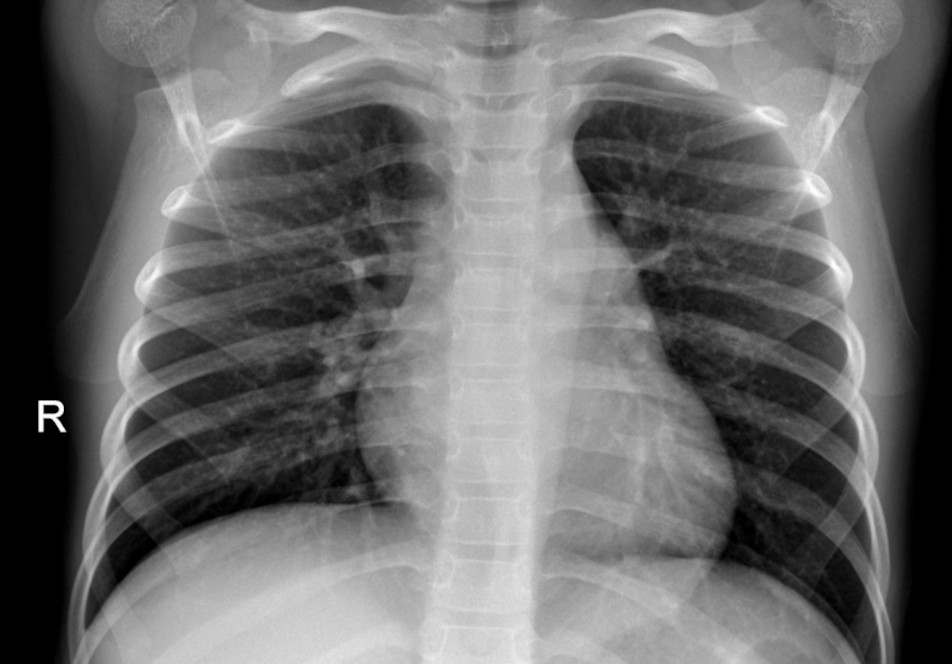
\includegraphics[width=.95\linewidth]{san}
  %\caption{1a}
  \caption{}
  \label{fig:snap1}
\end{subfigure}%
\begin{subfigure}{.32\textwidth}
  \centering
  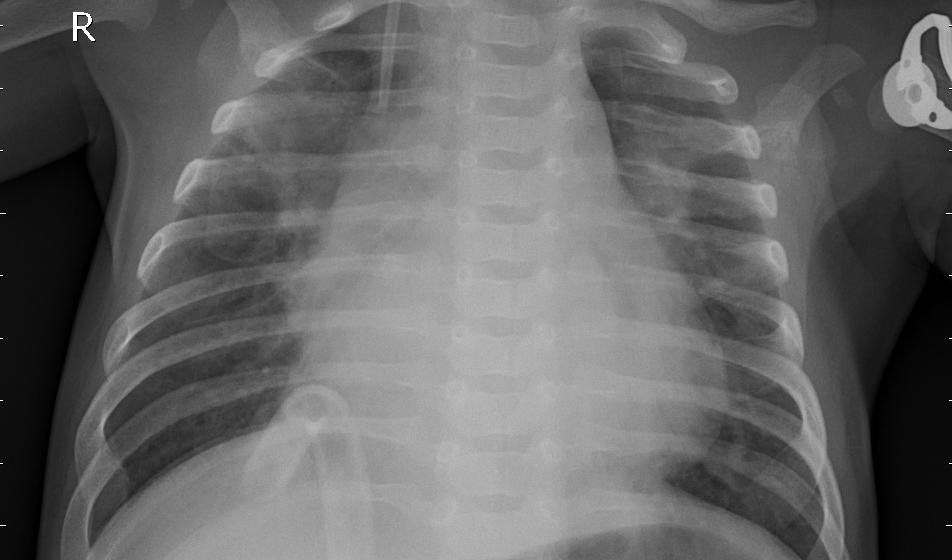
\includegraphics[width=.95\linewidth]{bacteria}
  %\caption{1a}
  \caption{}
  \label{fig:snap2}
\end{subfigure}%
\begin{subfigure}{.32\textwidth}
  \centering
  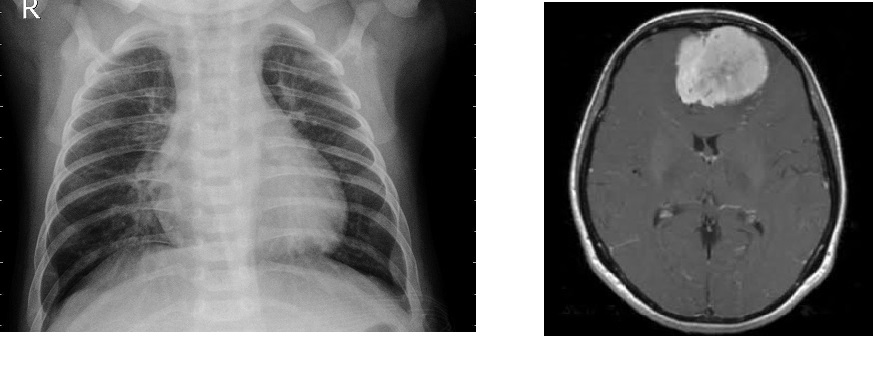
\includegraphics[width=.95\linewidth]{virus}
  %\caption{1b}
  \caption{}
  \label{fig:snap3}
\end{subfigure}
\caption{Si può notare come un soggetto sano (a) mostri polmoni senza aree di anormale opacità. L’immagine (b) è invece un caso di polmonite batterica che presenta il tipico consolidamento. (c) è un caso di polmonite virale che presenta un pattern interstiziale più diffuso in entrambi i polmoni.}
\label{fig:fig}
\end{figure} 

Il dataset è organizzato in 3 cartelle: una di Training (per l'addestramento stesso della rete), una di Testing (per testare le capacità di generalizzazione della rete) e una di Validation (per testare la bontà della rete e rilevare overfitting e/o underfitting in fase di addestramento). Ognuna di esse è organizzata così: 
\begin{itemize}
    \item 4,192 immagini per il training (1,082 casi normali, 3,110 di polmonite) 
    \item 1,040 immagini di validation (267 casi normali, 773 di polmonite) 
    \item 624 immagini per il testing (234 casi normali, 390 di polmonite) 
\end{itemize}
Il numero di immagini è sufficientemente grande per poter essere utilizzato per gli obiettivi preposti ricorrendo alle tecniche di deep learning per la computer vision di ambito biomedico. \\
Le proporzioni del dataset rispettano ampiamente gli standard che di solito si utilizzano per addestrare un modello di classificazione: un set di testing e uno di validation che è sono circa il (10-20)\% del totale, il resto è lasciato al training.
Si va adesso a sintetizzare quali sono stati i principali passaggi per l’implementazione della CNN.

\subsection{Setup iniziale}
Il primo step per realizzare il classificatore è l’importazione delle librerie necessarie per la manipolazione di tensori, per le operazioni matematiche e per la relizzazione di grafici (Pandas, NumPy, MatPlotLib), così come librerie di Keras per l’image preprocessing e oggetti di Deep Learning, tra cui:
\begin{itemize}
\item \lstinline{Sequential}, classe di Keras che permette di raggruppare layers, che non sono altro che i blocchi di base per la costruzione delle reti neurali, in uno stack lineare e realizzare così un oggetto di classe \lstinline{Model}, che è implementato in modo tale da riuscire a elaborare deduzioni una volta superata la fase di training; 
\item \lstinline{Conv2D}, classe che realizza la convoluzione spaziale sulle immagini 2D. Questo strato sfrutta un kernel di convoluzione il quale è coinvolto con lo strato in input per produrre un tensore in output. Se questo strato è usato per primo nel modello è necessario inserire come parametro la tupla rappresentante le dimensioni delle immagini in input. In questo strato è possibile scegliere il numero e le dimensioni del filtro, il valore dello stride (s=1 di default), il tipo di padding e altri parametri del caso; 
\item \lstinline{MaxPool2D}, realizza l’operazione di pooling, dunque è possibile anche qui scegliere la dimensione della pool, il valore dello stride, il tipo di padding...;
\item \lstinline{Flatten}, classe che permette di trasformare la feature map allo strato precedente in un vettore che viene dato in input alla ANN in seguito;
\item \lstinline{Dense}, classe che implementa un regolare strato di una NN. In sostanza è questo lo strato che implementa la somma pesata degli input con i pesi e il bias di cui si parlava nel capitolo 1. 
\end{itemize}

\subsection{Definizione degli iperparametri}
Successivamente sono stati fissati dei valori per gli iperparametri, ovvero quelle variabili poste all'inizio del codice, prima che il processo di apprendimento cominci. I valori degli iperparametri sono davvero importanti per l’accuratezza del modello e delle predizioni, infatti sono stati fatti variare alcune volte prima di arrivare alla migliore soluzione. I principali sono: 
\begin{itemize}
\item Le dimensioni di input dell’immagine, perchè è necessario che durante la fase di training vi sia un'uniformità delle dimensioni degli input;
\item il numero di epoche, cioè il numero di volte in cui l’algoritmo di apprendimento lavora sull’intero dataset prima di procedere con l’aggiornamento dei pesi. Sulla base di queste varia anche la durata dell’apprendimento. Infatti gli step di apprendimento per epoca sono pari alla divisione tra il numero di istanze del set di trainig e la batch size;
\item la batch size: è un iperparametro dell’algoritmo del gradiente discendente che indica il numero di campioni di training sui quali lavorare prima che venga fatto un aggiornamento dei pesi. Sia in questa esperienza sia in quella successiva si utilizza un algoritmo di apprendimento in modalità \emph{mini-batch} in quanto il dataset è abbastanza numeroso, ovvero si utilizza un valore di batch più grande rispetto a 1, così che non si vada ad aggiornare i valori dei pesi ogni volta che il sistema riceve un campione in input, quindi più del necessario, ottimizzando la durata dell'epoca e quindi del training. Di norma la batch size deve essere un valore che sia divisore del numero totale di immagini del dataset e nelle folders. 
\item il numero di feature maps: più che ne sono più caratteristiche differenti si possono andare a scovare ma allo stesso tempo aumenta anche il numero di parametri e se si vuole evitare il rischio di overfitting occorre aumentare la complessità del modello.
\item il numero di canali d'immagine utilizzati nel processo di learning: per le immagini RGB colorate tale parametro è pari a 3, mentre nel caso di immagini in scala di grigi vale 1. In tale caso le immagini sono digitali RGB ma vedremo che utilizzare solo un canale è la soluzione che porta ad una maggiore accuratezza.
\end{itemize}

Facendo riferimento agli iperparametri utilizzati per la costruzione del classificatore sono stati
 scelti tali iperparametri come i migliori per questa esperienza:\\
\lstinline{img_height = img_width = 600}\\
\lstinline{epochs = 10}\\
\lstinline{batch_size = 8}\\
\lstinline{hyper_featuremaps = 32}\\
\lstinline{hyper_channels = 1}\\
\lstinline{hyper_mode = 'grayscale'}\\

E’ stata utilizzata una dimensione per le immagini di 600 x 600 pixel associata a una batch size di 8
 affinchè lo spazio occupato in RAM non sia eccessivamente alto.  \\

\subsection{Definizione e compilazione del modello}
Per questa esperienza è stato utilizzato un modello di rete neurale convoluzionale semplice, che consiste di questi strati:\\
\begin{itemize}
\item 5 strati di Convoluzione/pooling: i primi 3 producono ognuno 32 feature maps con la convoluzione, 
generanti ognuna una feature map di pooling, per gli ultimi 2 sono stati invece utilizzati 64 filtri, 
così da produrre 64 feature maps anch’esse seguite da un’operazione di pooling. La convoluzione è stata performata
 con dei kernel di dimensione 3x3 e con una funzione di attivazione non lineare, cioè la ReLu. Nel capitolo precedente
  è stato indicato in parte il perchè questo tipo di funzione è quella maggiormente utilizzata in ambito di
   classificazione d’immagine, in quanto risolve in parte il problema della scomparsa del gradiente, uno dei 
   principali problemi del deep learning. Durante la fase di backpropagation i pesi degli strati in
    prossimità dell’input restano costanti o si aggiornano molto lentamente al contrario di quanto 
    accade per gli strati vicini all’output. Questo può provocare un rallentamento della rete ed è dovuto 
    alle funzioni di attivazione. Funzioni di attivazione come la sigmoide infatti sono funzioni a codominio
     limitato e hanno una derivata
      che presenta una regione di significatività piuttosto piccola, oltre la quale il valore della derivata stessa
       è molto piccolo. Per la regola della catena nella fase di backpropagation è necessario andare a fare un
        prodotto di derivate che è pari al numero di strati della rete neurale. A mano a mano che però si torna 
        indietro dall’output verso l’input però, moltiplicando valori molto vicini allo zero tra di loro si
         ottengono valori di aggiornamento dei pesi infinitesimi che comportano l'impossibilità per la rete
          di aggiornare i pesi correttamente, soprattutto quando si vanno ad utilizzare reti con più di due strati, e quindi quelle tipiche del deep learning.
           L'operazione di Max-pooling viene fatta con delle pool di dimensione
           2x2. Lo stride è stato lasciato quello di default a 1 e il padding scelto è il ‘same’, affinchè la
            dimensione dell’input sia uguale alla dimensione dell’output. 
\item Strato di flattening: necessario per introdurre la successiva ANN, connessa all’ultimo strato
 di pooling tramite un unico tensore unidimensionale.
\item 3 di strati completamente connessi rispettivamente di 128, 64 e 1 neuroni. 
L’ultimo strato consta di un solo neurone in quanto la classificazione è binaria. 
\end{itemize}

Tipicamente si parte sempre dall’utilizzare un numero di filtri più piccolo, come in questo caso 32,
 per poi andare ad aumentare a multipli di questa dimensione. 
Il modello è infine compilato usando il metodo \lstinline{compile()} usando la funzione di ottimizzazione Adam, 
algoritmo che si
 basa sull’idea del gradiente discendente ma che però elabora una stima adattativa dei momenti 
 del primo e del secondo ordine, permettendo una maggiore efficienza rispetto agli altri algoritmi
  a livello di costo computazionale per il training, a discapito di una conseguente minor capacità
   di generalizzazione. Inoltre Adam adatta il learning rate a seconda dei vari strati anche sulla base
    di quello che è il problema della scomparsa del gradiente di cui si è parlato sopra. \\
In fase di compilazione si sceglie anche la metrica, che permette di calcolare quanto spesso le label effettive
 coincidono con
 le predizioni fatte ed è dunque un parametro necessario per monitorare l’accuratezza e l’errore del modello.
  Una metrica di questo tipo viene settata col nome di \lstinline{'accuracy'}. 
  Per il calcolo dell’errore si usa una funzione di costo che in questo caso è chiamata \emph{binary crossentropy},
   (funzione di entropia incrociata binaria) poichè si va a fare una classificazione binaria.\\


   
    
\begin{python} %se voglio dividere in due pagine metto due \begin pyton separati
cnn = Sequential()
cnn.add(Conv2D(hyper_featuremaps, (3, 3), activation="relu", input_shape=(img_width, img_height, hyper_channels)))
cnn.add(MaxPooling2D(pool_size = (2, 2)))
cnn.add(Conv2D(hyper_featuremaps, (3, 3), activation="relu", input_shape=(img_width, img_height, hyper_channels)))
cnn.add(MaxPooling2D(pool_size = (2, 2)))
cnn.add(Conv2D(hyper_featuremaps, (3, 3), activation="relu", input_shape=(img_width, img_height, hyper_channels)))
cnn.add(MaxPooling2D(pool_size = (2, 2)))
cnn.add(Conv2D(hyper_featuremaps * 2, (3, 3), activation="relu", input_shape=(img_width, img_height, hyper_channels)))
cnn.add(MaxPooling2D(pool_size = (2, 2)))
cnn.add(Conv2D(hyper_featuremaps * 2, (3, 3), activation="relu", input_shape=(img_width, img_height, hyper_channels)))
cnn.add(MaxPooling2D(pool_size = (2, 2)))
cnn.add(Flatten())
cnn.add(Dense(activation = 'relu', units = 128))
cnn.add(Dense(activation = 'relu', units = 64))
cnn.add(Dense(activation = 'sigmoid', units = 1))
cnn.compile(optimizer = 'adam', loss = 'binary_crossentropy', metrics = ['accuracy'])
cnn.summary()

\end{python}
\begin{lstlisting}[caption= {Modello in Python utilizzato} ]
\end{lstlisting}

\newpage

\begin{python}
    Model: "sequential_1"
_________________________________________________________________
Layer (type)                 Output Shape              Param #   
=================================================================
conv2d_5 (Conv2D)            (None, 498, 498, 32)      320       
_________________________________________________________________
max_pooling2d_5 (MaxPooling2 (None, 249, 249, 32)      0         
_________________________________________________________________
conv2d_6 (Conv2D)            (None, 247, 247, 32)      9248      
_________________________________________________________________
max_pooling2d_6 (MaxPooling2 (None, 123, 123, 32)      0         
_________________________________________________________________
conv2d_7 (Conv2D)            (None, 121, 121, 32)      9248      
_________________________________________________________________
max_pooling2d_7 (MaxPooling2 (None, 60, 60, 32)        0         
_________________________________________________________________
conv2d_8 (Conv2D)            (None, 58, 58, 64)        18496     
_________________________________________________________________
max_pooling2d_8 (MaxPooling2 (None, 29, 29, 64)        0         
_________________________________________________________________
conv2d_9 (Conv2D)            (None, 27, 27, 64)        36928     
_________________________________________________________________
max_pooling2d_9 (MaxPooling2 (None, 13, 13, 64)        0         
_________________________________________________________________
flatten_1 (Flatten)          (None, 10816)             0         
_________________________________________________________________
dense_3 (Dense)              (None, 128)               1384576   
_________________________________________________________________
dense_4 (Dense)              (None, 64)                8256      
_________________________________________________________________
dense_5 (Dense)              (None, 1)                 65        
=================================================================
Total params: 1,467,137
Trainable params: 1,467,137
Non-trainable params: 0

\end{python}
\begin{lstlisting}[caption = {Riepilogo del modello. La colonna \lstinline{layer} indica il tipo di strato di cui si tratta. La colonna output mostra la tupla con le dimensioni dello strato in uscita, con una dimensione
    in più \lstinline{None} che è aggiunta per ospitare la batch size. La terza colonna \lstinline{Param \#} indica il numero di pesi all'interno della rete, i quali possono essere distinti in addestrabili, cioè quelli che vengono aggiornati durante la fase di backpropagation, e quelli per cui questo non vale per motivi di regolarizzazione della rete. Il numero totale di parametri si trova \lstinline{(kernel_height*kernel_width*input_filters*output_filters) + 
    output_filters}. Ad esempio nel primo strato si avra 3*3*32*1+32=320.}]
  
\end{lstlisting}

\subsection{Creazione dei set di training e validation traminte l’uso dell’image flowing}
Tramite l’utilizzo della classe di Keras  \lstinline{ImageDataGenerator()} è possibile andare a caricare le
 immagini di training, testing e validation andando a richiamare su tali generatori il metodo  
 \lstinline{flowFromDirectory()} che è in grado di ritornare un oggetto di tipo DataFrameGenerator
 costituito da una tupla (X , y) dove X è un NumPy array contenente un numero di immagini pari alla 
   \lstinline{batch size} e della dimensione pari a  \lstinline{image_width}x\lstinline{image_height}indicata e 
   y è anch’esso
    un NumPy array che però contiene le label corrispondenti alle immagini prodotte. L’utilizzo di
     questa funzione è possibie perchè il dataset è strutturato in partenza in un dataset di trainining, 
     validation e testing. Inoltre tale funzione genera i set provvedendo a fare uno shuffle di tutte le immagini
      sia di training sia di  validation, mentre per il set di testing è stato inserito  \lstinline{Shuffle = False}
       così da poter testare la capacità di generalizzazione della rete e confrontare le predizioni con i risultati 
       effettivi. \\
 \lstinline{ImageDataGenarator} è una classe che permette anche di utilizzare tecniche di \emph{augmentation}
  per ampliare il dataset. Tali tecniche prevedono di andare a costruire versioni modificate delle immagini stesse. 
  Infatti il dataset, pur essendo numeroso, non lo è al punto tale da rendere sufficientemente buona l’esperienza
   di image processing. Questa mancanza può essere pertanto colmata andando ad ampliare il dataset con immagini
    che possano arricchire l’esperienza di training del modello. Tali immagini possono essere modificate in vari
     modi, ma non tutti questi sono utili nel caso di interesse: infatti alcune tecniche possono generare rumore 
     aggiuntivo e ‘’confondere’’ il sistema nella ricerca dei pattern per la rilevazione della polmonite.
     Infatti è differente classificare immagini biomedicali come i raggi
     X per capire se vi è o meno una polmonite rispetto ad una classificazione di immagini come quelli di 
     cani o di gatti. Infatti, mentre un gatto può essere visto da varie angolazioni e ciò può essere
      utile al fine di distinguerlo da un cane, operare una rotazione troppo elevata per andare a riconoscere 
      l’opacità dei polmoni in un’immagine a raggi X, non va ad arricchire il dataset, ma può portare
       addirittura a un peggioramento dell’accuratezza del modello. Nell’esperienza è stato fatto un
        training del modello dapprima senza l’utilizzo di tecniche di image augmentation, per poi confrontarlo
         con un altro training in cui è stato ampliato il dataset. \\

      Occorre pertanto scegliere accuratamente quali parametri inserire. Le tecniche che sono risultate essere utili in questo caso sono:
      \begin{itemize}
        \item \textbf{Rescaling}: dato che è stata definita la modalità di colorazione 'grayscale' ogni pixel di 
        ogni immagine avrà un valore che sta nel range [0,255] che con questa tecnica diviene compreso tra 0 e 1. 
        Un primo beneficio è che così tutte le immagini vengono trattate alla stessa maniera. 
        Infatti è possibile che alcune immagini abbiano un range alto di valori dei pixel, altre più basso,
         ma entrambe condividono poi lo stesso modello e learning rate per il training. 
        In generale è bene fare in modo che il range di valori sia compreso tra 0 e 1 così che ogni immagine
         contribuisca nella maniera più uniforme possibile per il calcolo della funzione di perdita totale e 
         quindi per l'aggiornamento dei pesi. 
        \item \textbf{Rotazione}: è stato appurato che un piccolo range di rotazione per le immagini possa essere
         utile a migliorare le capacità di generalizzazione del sistema, proprio perchè molto spesso nella pratica clinica
         le radiografie possono essere lievemente ruotate a causa dei movimenti del paziente. Il range utilizzato in questo caso è tra i 
         -5$^\circ$  e i 5$^\circ$.
         \item \textbf{Zoom}: come nel caso della rotazione, è prassi che vi siano immagini in cui il torace del paziente sia posizionato
         più o meno vicino al dispositivo che elabora l'immagine. Quindi un piccolo range di variazione dello zoom delle immagini (in questo caso è stato scelto 0.1) 
         può essere utile. 
        
      \end{itemize}


      
      \begin{figure}[H]
        \centering
        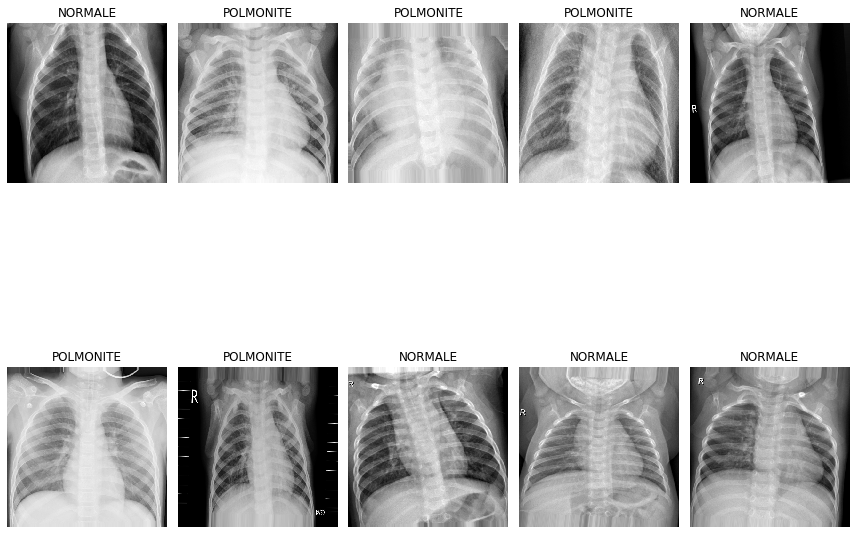
\includegraphics[width=0.9\textwidth]{Figures/best-augmented-images-pneumonia.png}
        \caption{\small{
        Campioni di immagini del dataset di training sui quali sono state aggiunte le tecniche sopra citate.
        } % end small
        } % end caption
        \label{fi:dcalc}
    \end{figure}
      
     
\subsection{Fase di fitting}
Dopo aver compilato e configurato il modello si passa alla fase di \emph{fitting}, cioè la fase di addestramento
 vera e propria. Il modello viene dunque allenato tramite le immagini del set di training, con un aggiornamento
  dei pesi che viene fatto per ogni gruppo di campioni pari alla \lstinline{batchsize}. Il set di training viene rivisto
   per un totale di 20 epoche, anche se dopo 10 la capacità di training risulta essere stagnante.
    Una volta captato questo è stata usata la funzione di callback \lstinline{EarlyStopping()} che ha fermato il
     training non appena risultava esserci overfitting. 
   Il metodo  \lstinline{fit()} ci permette anche di scegliere l’insieme di validation su cui la rete 
   può generalizzare. Ciò fa sì che non solo si possa monitorare l'accuratezza nel training, ma anche la
    capacità di generalizzazione della rete, cercando di capire se questa sta andando in overfitting, 
    underfitting o se il trade-off tra le due è accettabile, così da agire di conseguenza 
    per poterla migliorare. Si può anche definire una lista di chiamate (callbacks) per 
    customizzare il training, come definire un checkpoint dove salvare il modello così 
    da poterlo utilizzare successivamente per elaborare nuove predizioni,
     senza necessità di allenarlo nuovamente.  Inoltre è stata utilizzata una funzione che riduce il 
     valore del learning rate del 30\% automaticamente ogni due epoche in quanto molto spesso 
     il modello beneficia di ciò se l’apprendimento stagna. 
     %(Aprire parentesi nei capitoli precedenti di come il lr influenza l’apprendimento)
In questo caso il modello è stato allenato sull’insieme di training e validation definito dal dataset stesso.
 Il set di testing è l’insieme di immagini sulle quali si va a fare la valutazione finale.
  \begin{figure}[H]
    \begin{subfigure}{0.55\textwidth}
      \centering
      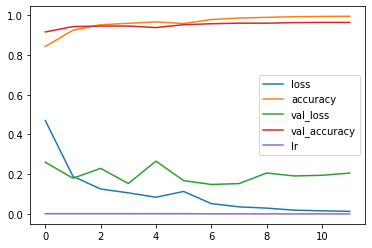
\includegraphics[width=0.95\linewidth]{Figures/history-pneumonia-no-aug.png}
      %\caption{1a}
      \caption{}
      \label{fig:snap1}
    \end{subfigure}%
    \begin{subfigure}{0.55\textwidth}
      \centering
      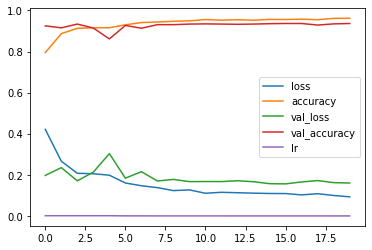
\includegraphics[width=.95\linewidth]{Figures/history-pneumonia-aug.png}
      %\caption{1a}
      \caption{}
      \label{fig:snap2}
    \end{subfigure}%
    \caption{In entrambe le figure è possibile osservare la curva ROC sul training e sul set di validation. Lo scopo è quello che la curva arancione tenda ad un gradino di ampiezza unitaria.}
    \label{fig:fig}
\end{figure} 
Alla fine si ottengono questi risultati andando a richiamare \lstinline{cnn.evaluate(test)}:
\begin{itemize}
  \item Per il caso senza modifiche al set di training risulta che l'accuracy sul training è pari al (99.61 $\pm$ 0.01)\% e quella sull'insieme di validation è del (94.44 $\pm$ 0.01)\%.
  \item  Per il caso con le modifiche al set di training risulta che l'accuracy sul training è pari al (96.99 $\pm$ 0.01)\% e quella sull'insieme di validation è del (94.61 $\pm$ 0.01)\%.
  
\end{itemize}


\subsection{Predizioni}
Infine occorre osservare come il sistema riesce a generalizzare sull’insieme di test. 
Dato che la funzione di attivazione dello strato finale del modello è la sigmoide, 
il valore dell’output starà in un range compreso tra 0 e 1 corrispondente alla probabilità che l’immagine
 su cui è stata fatta la predizione presenti polmonite o meno. 
Se si vogliono quantificare i falsi positivi e i falsi negativi occorre vedere se l’output della 
rete è superiore o inferiore a 0.5  e di conseguenza predire se si tratta di polmonite o meno.
 É possibile visualizzare la matrice di confusione\footnote{É un modo per visualizzare in maniera 
 diretta il numero di predizioni corrette/falsi-negativi/falsi-positivi}. 
 Le tabelle 5.1 e 5.2 rappresentano dei report di classificazione in cui è possibile osservare 3 diverse voci:
\begin{itemize}
  \item Precision = (Predizioni corrette) / (Predizioni corrette + Falsi positivi)
  \item Recall = Predizioni corrette / (Predizioni corrette + Falsi negativi)
  \item F1 = (2 * Precision * Recall) / (Precision + Recall)
\end{itemize}
  % Please add the following required packages to your document preamble:
% 



  \begin{table}[hb!]
  \begin{tabular}{@{}l|llll@{}}
    \toprule
                     & \textbf{precision} & \textbf{recall} & \textbf{f1-score} & \textbf{support} \\ \midrule
  \textbf{NORMALE}   & 0.99               & 0.36            & 0.53              & 234              \\
  \textbf{POLMONITE} & 0.72               & 1.00            & 0.84              & 390              \\ \midrule
  accuracy           &                    &                 & 0.76              & 624              \\
  macro avg          & 0.85               & 0.68            & 0.68              & 624              \\
  weighted avg       & 0.82               & 0.76            & 0.72              & 624              \\ \bottomrule
  \end{tabular}
  \caption{}
\end{table} 
  
  

\begin{table}[hb!]
  \begin{tabular}{@{}l|llll@{}}
  \toprule
                     & \textbf{precision} & \textbf{recall} & \textbf{f1-score} & \textbf{support} \\ \midrule
  \textbf{NORMALE}   & 0.97               & 0.85            & 0.90              & 234              \\
  \textbf{POLMONITE} & 0.91               & 0.98            & 0.95              & 390              \\ \midrule
  accuracy           &                    &                 & 0.93              & 624              \\
  macro avg          & 0.94               & 0.92            & 0.93              & 624              \\
  weighted avg       & 0.94               & 0.93            & 0.93              & 624              \\ \bottomrule
  \end{tabular}
  \caption{}
\end{table}

In sintesi l'accuratezza del modello sull'insieme di test vale:
\begin{itemize}
  \item  (75.80 $\pm$ 0.01)\% nella prima esperienza;
  \item  (93.27 $\pm$ 0.01)\% nella seconda.
\end{itemize}
Dunque sembra che, nonostante nella prima esperienza si abbia ottenuto un'accuratezza migliore sul training, 
poi le capacità di generalizzazione sono migliori quelle ottenute con la seconda.
 Ciò significa che nel primo training si è avuto un problema di overfitting. 


 \begin{figure}[H]
        \begin{subfigure}{0.55\textwidth}
          \centering
          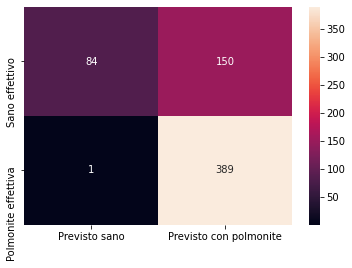
\includegraphics[width=0.95\linewidth]{Figures/conf-matrix-no-aug.png}
          %\caption{1a}
          \caption{}
          \label{fig:snap1}
        \end{subfigure}%
        \begin{subfigure}{0.55\textwidth}
          \centering
          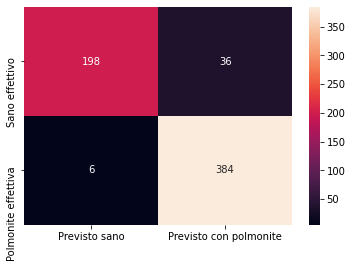
\includegraphics[width=.95\linewidth]{Figures/conf-matrix-pneumonia-aug.png}
          %\caption{1a}
          \caption{}
          \label{fig:snap2}
        \end{subfigure}%
        \caption{ Matrici di confusione ottenute. (a) è la matrice di confusione del modello con il set di
         training lasciato come l'originale. 
        Si può vedere che vi sono molti errori nel prevedere il soggetto sano. \\
        (b) è la matrice di confusione con il set di training modificato come nella Figura 5.2. 
        In questo caso vi sono pochissimi errori di predizione.
        }
        \label{fig:fig}
\end{figure} 


\begin{figure}[H]
  \centering
  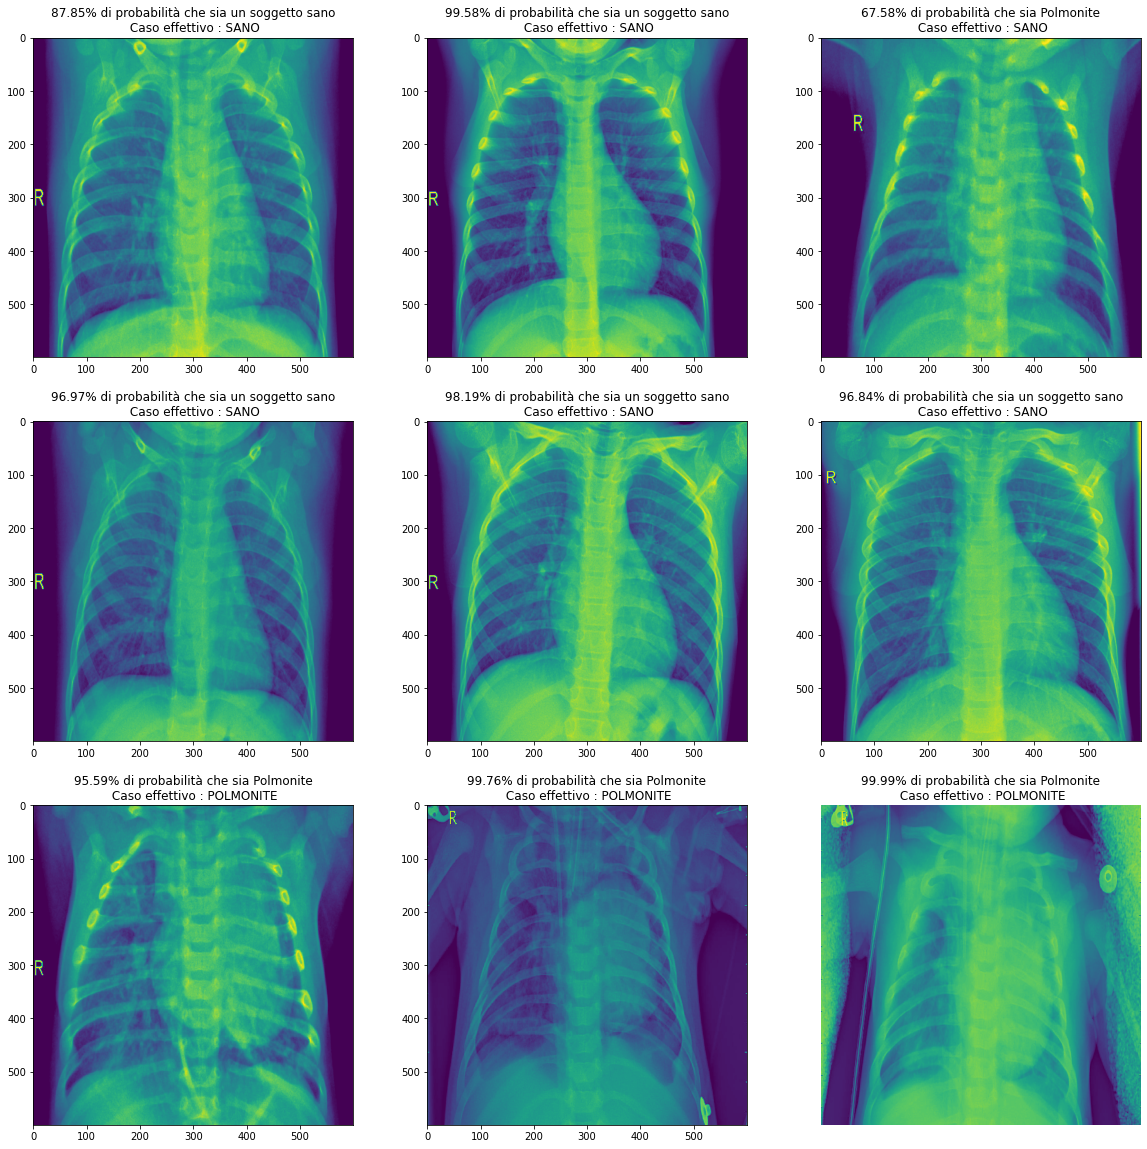
\includegraphics[width=0.9\textwidth]{Figures/test-results-pneumonia-600.png}
  \caption{\small{Dimostrazione di alcune previsioni.
  } % end small
  } % end caption
  \label{fi:dcalc}
\end{figure}
 
 
 
\subsection{Considerazioni finali}
La rete addestrata con il dataset ampliato risulta produrre buoni risultati. 
In prima istanza sicuramente grazie all’accuratezza del dataset, ma anche grazie a degli iperparametri ben scelti. 
Sono state in effetti fatte delle prove con image size di dimensioni 400x400, 500x500, 600x600 e batch size = 8, 16, 32 ,
 ma la migliore accuratezza di generalizzazione si ha con gli iperparametri della sezione 5.2.3. Risultati ragionevoli 
 sono stati trovati dopo 10 epoche, anche se è stato fatto un addestramento anche con 25 e 50 epoche
 , ma ciò risultava inutile in quanto dalla decima epoca in poi l’accuratezza 
 del modello rimane costante e non migliora. Per evitare ciò è stato utilizzato l’Early Stopping che ha
  appunto fermato il modello intorno alla decima epoca. 
Inoltre è stato provato anche ad aumentare il numero dei canali d’immagine
 da 1 a 3 ma ciò non ha fatto altro che peggiorare le prestazioni. Probabilmente 
 ciò è dovuto al fatto che per rilevare una polmonite la scala di grigi evidenzia maggiormente l’opacità del polmone. 
Sicuramente se il classificatore dovesse essere utilizzato in uno studio radiologico,
 sarebbe un buon mezzo di supporto in quanto il numero di falsi negativi è minore rispetto
  a quello dei falsi positivi ed è molto piccolo (clinicamente è meglio che sia diagnosticato 
  un falso positivo piuttosto che un falso negativo!). Sotto si mostrano i risultati ottenuti con iperparametri
   differenti (eccetto il numero di epoche in tutti i casi pari a 20), con le modifiche apportate al set di training della sezione 5.2.5
    e che hanno portato alla scelta di quelli alla sezione 5.2.3.

    \begin{table}[hb!]
      \begin{tabular}{l|lll}
      \hline
                                                                                                         & \multicolumn{1}{l|}{\textbf{training accuracy}} & \multicolumn{1}{l|}{\textbf{validation accuracy}} & \textbf{test accuracy} \\ \hline
      \textbf{\begin{tabular}[c]{@{}l@{}}batch = 16\\ image size = 500x500\\ channels = 1\end{tabular}}  & 95.99\%                                         & 93.65\%                                           & 91.98\%                \\ \hline
      \textbf{\begin{tabular}[c]{@{}l@{}}batch = 32\\ image size = 400x400\\ channels = 1\end{tabular}}  & 95.94\%                                         & 95.00\%                                           & 91.5\%                 \\ \hline
      \textbf{\begin{tabular}[c]{@{}l@{}}batch = 8\\ image size = 600 x 600\\ channels = 1\end{tabular}} & 96.49\%                                         & 94.61\%                                           & 93.26\%                \\ \hline
      \textbf{\begin{tabular}[c]{@{}l@{}}batch = 8\\ image size = 600 x 600\\ channels = 3\end{tabular}} & 96.32\%                                         & 93.94\%                                           & 92.62\%                \\ \hline
      \end{tabular}
      \end{table}
\newpage
\section{CNN per la classificazione di risonanze magnetiche cerebrali}





\chapter{Conclusioni}

Al termine delle due esperienze è stato possibile andare a classificare immagini biomedicali utilizzando reti neurali 
convoluzionali ed ottenere buoni risultati sia implementando e allenando la rete partendo da 0, sia utilizzando un modello
precedentemente allenato. \\
É stato visto inoltre quanto sia necessario un buon dataset come punto di partenza così come vi debba essere un equilibrio tra le dimensioni
del set di training e quello del set di testing, quelle degli iperparametri, facendo attenzione anche all'architettura della CNN scelta,
 così che non presenti troppi parametri rispetto alla complessità del problema di interesse, ma nemmeno che questi siano insufficienti.\\
La difficoltà  principale nell'andare a realizzare sistemi come questi sta proprio nel dosare nella maniera più corretta tutti questi fattori, ed è necessario 
per riuscirci compiere una quantità molto elevata di training, applicando la tecnica conosciuta come \emph{trial and error}. 

É stato visto come costruire tali modelli richieda diversi step, partendo da una corretta analisi del dataset, 
elaborare i primi risultati fino a trovare gli iperparametri ottimali in seguito a vari tentativi e procedere con il fine-tuning della rete di conseguenza,
 ampliando il dataset se necessario.
Sono state passate in rassegna le tecniche per estendere il set di training di maggior uso fino a capire che nel caso di immagini biomedicali
è bene non andare a caso nella scelta di queste e che tutto dipende da quelli che sono i pattern significativi da riconoscere.
 
É bene scegliere trasformazioni che non vadano a rivoluzionare troppo gli schemi di immagine veri e propri, dunque le trasformazioni geometriche
possono essere utili solo se fatte nella misura giusta da non portare alla creazione di esempi anatomicamente incorretti
 e ciò richiede sforzo nell'andare a ricercare quale siano le migliori. 
Andare ad aggiungere limitatamente trasfomazioni \emph{pixel-wise} nel caso del secondo dataset e delle leggere rotazioni e zoom alle immagini nel primo dataset 
sono state i modi in cui sono stati ottenuti i migliori risultati. \\
Ovviamente tutto questo funziona se il modello è ben strutturato, altrimenti questo potrebbe fare da collo di bottiglia al training.\\
Infine questa esperienza mostra come l'utilizzo delle CNN possa essere esteso a vari tipi di classificazione e che 
modelli come quelli illustrati possano essere utilizzati per altri tipi di dataset affini. É sicuramente possibile sfruttare
i training fatti alle reti neurali sui due dataset e riutilizzarne i pesi per training successivi
 per l'identificazione di altre patologie, 
ad esempio andando a fare un'ulteriore distinzione
tra polmonite virale o batterica in riferimento al modello ottenuto nella prima esperienza oppure per andare a
 riconoscere malattie neurologiche che comportano una mutazione anomala dell'encefalo (che quindi possono essere riconoosciute tramite RM), 
 come ad esempio quelle neurodegenerative (es. Alzehimer), usando il secondo sistema.
 
 É possibile infatti durante ogni training salvare il modello allenato in un file e riutilizzarlo quando si vuole.\\
 Si riportano adesso le curve \emph{ROC (Receiver Operating Characteristics)} per mostrare 
 la validità dei sistemi implementati.  
 La curva ROC~\cite{Roc} è uno schema di rappresentazione grafica che permette di valutare l’efficienza 
 di un classificatore binario. L’analisi di della curva ROC è un metodo statistico utilizzato spesso in ambito biomedico. Essa rappresenta il metodo d’elezione 
per validare un test diagnostico. 
La curva ROC viene costruita mettendo in ascissa la \emph{specificità} ($\frac{TN}{TN+FP}$) e in ordinata la \emph{sensibilità} ($\frac{TP}{TP+FN}$, corrisponde a quella che nel capitolo 5 è stata definita come \emph{recall}) per tutti i possibili valori del test diagnostico. L’area sotto la curva ROC, \emph{area
under curve (AUC)}, è una misura quantitativa della bontà del classificatore, che può assumere valori tra 0.5 e
 1.0. Se il valore della AUC è compreso tra 0,9 e 1.0 significa che il classificatore è altamente accurato e possiede alto potere discriminante.
 Tanto maggiore è l’area sotto la curva (cioè tanto
più la curva si avvicina al vertice in alto a sinistra del grafico, quanto più  somiglia ad un gradino) tanto maggiore è il potere discriminante della rete.\\



\begin{figure}[hb!]
  \begin{subfigure}{0.5\textwidth}
    \centering
    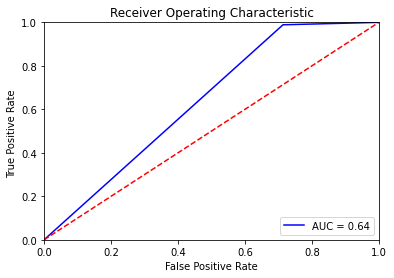
\includegraphics[width=1\textwidth]{Figures/roc-pneumonia-no-aug.png}
    %\caption{1a}
    \caption{}
    \label{fig:snap1}
  \end{subfigure}%
  \begin{subfigure}{0.5\textwidth}
    \centering
    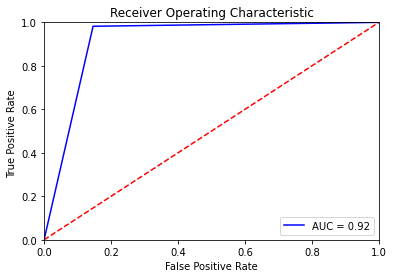
\includegraphics[width=1\textwidth]{Figures/roc-pneumonia-aug.png}
    %\caption{1a}
    \caption{}
    \label{fig:snap2}
  \end{subfigure}%
  \caption{Confronto della caratteristica ROC tra il sistema per la rilevazione della polmonite senza applicare le modifiche al set di training (a)
  e quella del sistema allenato sul set ampliato (b). Il codice di realizzazione può essere visto nel Code Listing 7.1.
  }
  \label{fig:fig}
\end{figure} 



\begin{figure}[hb!]
    \begin{subfigure}{0.5\textwidth}
      \centering
      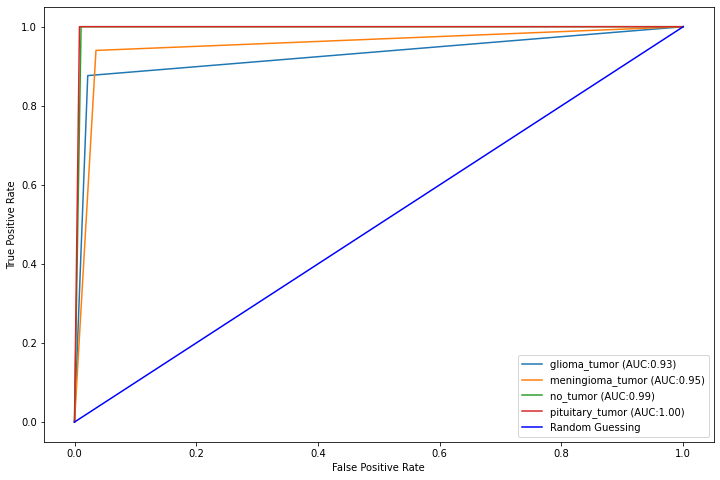
\includegraphics[width=1\textwidth]{Figures/roc-alexnet.png}
      %\caption{1a}
      \caption{}
      \label{fig:snap1}
    \end{subfigure}%
    \begin{subfigure}{0.5\textwidth}
      \centering
      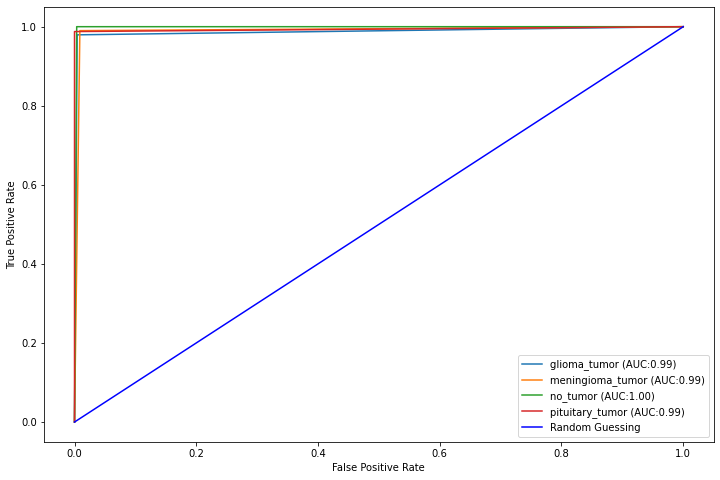
\includegraphics[width=1\textwidth]{Figures/ROC-pretrained.png}
      %\caption{1a}
      \caption{}
      \label{fig:snap2}
    \end{subfigure}%
    \caption{Confronto tra la caratteristica ROC del modello \emph{2.} con rumore gaussiano e del modello \emph{3.} per il dataset delle RM.
    (a) mostra una AUC di 0.96, (b) dello 0.99. Il codice di realizzazione può essere visto nel Code Listing 7.2.
    }
    \label{fig:fig}
\end{figure} 


 

\chapter{Codice}

%Si riporta il codice Python utilizzato per il training del sistema per la classificazione dei raggi X e successivamente quello per la diagnostica delle RM.

\begin{lstlisting}[basicstyle=\tiny, language=Python, caption=Esempio di implementazione di una CNN per la classificazione di raggi-X.~\cite{dspneum} ]
#Si importano le principali librerie
import matplotlib.pyplot as plt #per la visualizzazione
import numpy as np              #per gestire gli array
import pandas as pd             #per gestire i dati
from tensorflow.keras.models import Sequential
from tensorflow.keras.layers import Dense,Conv2D,Flatten,MaxPooling2D
from tensorflow.keras.callbacks import EarlyStopping,ReduceLROnPlateau
from sklearn.utils.class_weight import compute_class_weight
from sklearn.metrics import classification_report,confusion_matrix
import sklearn.metrics as metrics #per fare le previsioni
import seaborn as sns 
import scikitplot as skplt

#Si definiscono le directory per il training, testing e validation
train_path = './pneumonia/train'
test_path = './pneumonia/test'
valid_path = './pneumonia/val'

#Si definiscono gli iperparametri
batch_size = 16
img_height = 500
img_width = 500
channels = 1
hyper_epochs = 20

#Si applicano le teniche di image preprocessing di cui si parla nella sezione 5.2.5 al set di training e testin
from tensorflow.keras.preprocessing.image import ImageDataGenerator# Create Image Data Generator for Train Set
image_gen = ImageDataGenerator( rescale = 1./255,
                                rotation_range = 5,
                                zoom_range = 0.2)                            
test_data_gen = ImageDataGenerator(rescale = 1./255)

train = image_gen.flow_from_directory(
      train_path,
      target_size=(img_height, img_width),
      color_mode='grayscale',
      class_mode='binary',
      batch_size=batch_size
      )
test = test_data_gen.flow_from_directory(
      test_path,
      target_size=(img_height, img_width),
      color_mode='grayscale',
      shuffle=False, 
    #si setta shuffle=False per non avere problemi di indicizzazione quando si va a fare il test
      class_mode='binary',
      batch_size=batch_size
      )
valid = test_data_gen.flow_from_directory(
      valid_path,
      target_size=(img_height, img_width),
      color_mode='grayscale',
      class_mode='binary', 
      batch_size=batch_size
      )

#codice per stampare alcuni campioni del set di training che andranno in input alla rete
plt.figure(figsize=(12, 12))
for i in range(0, 10):
    plt.subplot(2, 5, i+1)
    for X_batch, Y_batch in train:
        image = X_batch[0]        
        dic = {0:'NORMALE', 1:'POLMONITE'}
        plt.title(dic.get(Y_batch[0]))
        plt.axis('off')
        plt.imshow(np.squeeze(image),cmap='gray',interpolation='nearest')
        break
plt.tight_layout()
plt.show()

#Si definisce il modello
cnn = Sequential()
cnn.add(Conv2D(32, (3, 3), activation="relu", input_shape=(img_width, img_height, channels)))
cnn.add(MaxPooling2D(pool_size = (2, 2)))
cnn.add(Conv2D(32, (3, 3), activation="relu", input_shape=(img_width, img_height, channels)))
cnn.add(MaxPooling2D(pool_size = (2, 2)))
cnn.add(Conv2D(32, (3, 3), activation="relu", input_shape=(img_width, img_height,  channels)))
cnn.add(MaxPooling2D(pool_size = (2, 2)))
cnn.add(Conv2D(64, (3, 3), activation="relu", input_shape=(img_width, img_height, channels)))
cnn.add(MaxPooling2D(pool_size = (2, 2)))
cnn.add(Conv2D(64, (3, 3), activation="relu", input_shape=(img_width, img_height, channels)))
cnn.add(MaxPooling2D(pool_size = (2, 2)))
cnn.add(Flatten())
cnn.add(Dense(activation = 'relu', units = 128))
cnn.add(Dense(activation = 'relu', units = 64))
cnn.add(Dense(activation = 'sigmoid', units = 1))
#Si compila il modello applicando l'ottimizzatore e la funzione di errore 
#sulla quale si basa l'algoritmo di backpropagation
cnn.compile(optimizer = 'adam', loss = 'binary_crossentropy', metrics = ['accuracy'])
cnn.summary()

#Si definiscono le callbacks che il sistema sfrutta nel training
from tensorflow.keras.callbacks import EarlyStopping, ReduceLROnPlateau, TensorBoard, ModelCheckpoint
early = EarlyStopping(monitor= 'val_loss', mode='min', patience=5)
learning_rate_reduction = ReduceLROnPlateau(monitor='val_loss', patience = 2, verbose=1,factor=0.3,min_delta = 0.001, min_lr=0.000001)
checkpoint = ModelCheckpoint("my model.h5",monitor="val_accuracy",save_best_only=True,mode="auto",verbose=1)
callbacks_list = [ early, learning_rate_reduction, checkpoint]

#Si vanno ad assegnare i valori dei pesi per ogni classe a seconda della cardinalita 
#degli elementi presenti in essa. 
#Dunque il modello assegna automaticamente i pesi della classe in maniera inversamente
#proporzionale alla frequenza degli elementi in una classe
weights = compute_class_weight('balanced', np.unique(train.classes), train.classes)
cw = dict(zip( np.unique(train.classes), weights))
print(cw)

#Si fa il fitting
history = cnn.fit(train,epochs=hyper_epochs, validation_data=valid, class_weight=cw, callbacks=callbacks_list)

#Si crea un grafico dell'andamento 
pd.DataFrame(cnn.history.history).plot()

#Si controlla l'accuratezza del test
test_accu = cnn.evaluate(test)
print('The testing accuracy is :',test_accu[1]*100, '%')
test_accu = cnn.evaluate(train)
print('The training accuracy is :',test_accu[1]*100, '%')
test_accu = cnn.evaluate(valid)
print('The validation accuracy is :',test_accu[1]*100, '%')

#Si fanno le previsioni
preds = cnn.predict(test,verbose=1)
predictions = preds.copy()
predictions[predictions <= 0.5] = 0
predictions[predictions > 0.5] = 1

#si genera la matrice di confusione
cm = pd.DataFrame(data=confusion_matrix(test.classes, predictions, labels=[0, 1]),index=["Sano effettivo", "Polmonite effettiva"],
columns=["Previsto sano", "Previsto con polmonite"])
sns.heatmap(cm,annot=True,fmt="d")

#si stampa un report di classificazione
print(classification_report(y_true=test.classes,y_pred=predictions,target_names =['NORMALE','POLMONITE']))

#Si stampano alcuni esempi di immagini con associata la classe prevista e la probabilita con cui 
#la previsione sia corretta, associata alla diagnosi effettiva (La figura 5.6 mostra l'output ottenuto)
test.reset()
x=np.concatenate([test.next()[0] for i in range(test.__len__())])
y=np.concatenate([test.next()[1] for i in range(test.__len__())])
print(x.shape)
print(y.shape)#this little code above extracts the images from test Data iterator without shuffling the sequence
# x contains image array and y has labels 
dic = {0:'SANO', 1:'POLMONITE'}
plt.figure(figsize=(20,20))
for i in range(0+228, 9+228):
  plt.subplot(3, 3, (i-228)+1)
  if preds[i, 0] >= 0.5: 
      out = ('{:.2%} di probabilita che sia Polmonite'.format(preds[i][0]))
      
      
  else: 
      out = ('{:.2%} di probabilita che sia un soggetto sano'.format(1-preds[i][0]))
  plt.title(out+"\n Caso effettivo : "+ dic.get(y[i]))    
  plt.imshow(np.squeeze(x[i]))
plt.axis('off')
plt.show()


data = []     # archivia tutte le batch di immagini prodotte nell'insieme di test
labels = []   # archivia le label associate alle immagini dell'array sopra
max_iter = 100  # massimo numero di iterazioni, a seconda della batch size e della dimensione del dataset
i = 0
for d, l in test:
    data.append(d)
    labels.append(l)
    i += 1
    if i == max_iter:
        break
data = np.array(data)
data = np.reshape(data, (data.shape[0]*data.shape[1],) + data.shape[2:])

labels = np.array(labels)
labels = np.reshape(labels, (labels.shape[0]*labels.shape[1],) + labels.shape[2:])

# si calcolano i falsi positivi e i falsi negativi per produrre la caratteristica ROC
preds = cnn.predict(data)
preds[preds <= 0.5] = 0
preds[preds > 0.5] = 1

fpr, tpr, threshold = metrics.roc_curve(labels, preds)
roc_auc = metrics.auc(fpr, tpr)

plt.title('Receiver Operating Characteristic')
plt.plot(fpr, tpr, 'b', label = 'AUC = %0.2f' % roc_auc)
plt.legend(loc = 'lower right')
plt.plot([0, 1], [0, 1],'r--')
plt.xlim([0, 1])
plt.ylim([0, 1])
plt.ylabel('True Positive Rate ')
plt.xlabel('False Positive Rate')
plt.show()
\end{lstlisting}


\begin{lstlisting}[basicstyle=\tiny, language=Python, caption=Esempio di implementazione di AlexNet per la classificazione di RM con l'aggiunta di rumore al set di training.~\cite{dsbrain} ]
#Si importano le librerie principali
from keras.callbacks import TensorBoard
import matplotlib.pyplot as plt
import numpy as np
import pandas as pd
import seaborn as sns
import cv2
import tensorflow as tf
from tensorflow.keras.preprocessing.image import ImageDataGenerator
from tqdm import tqdm
import os
from pathlib import Path
import itertools
from sklearn.utils import shuffle
from keras import Sequential
from sklearn.model_selection import train_test_split
from tensorflow.keras.applications import EfficientNetB0
from tensorflow.keras.callbacks import EarlyStopping, ReduceLROnPlateau, TensorBoard, ModelCheckpoint
from sklearn.metrics import classification_report,confusion_matrix
import ipywidgets as widgets
import io
from keras.layers import Flatten,Dense,BatchNormalization,Activation,Dropout
from tensorflow.keras.utils import to_categorical
from PIL import Image
from IPython.display import display,clear_output
from warnings import filterwarnings
from tensorflow import keras 
from tensorflow.keras import layers
from tensorflow.keras.models import Sequential
from tensorflow.keras.layers import Dense,Conv2D,Flatten,MaxPooling2D, Input
from tensorflow.keras.callbacks import EarlyStopping,ReduceLROnPlateau
from keras.regularizers import l2
from tensorflow.keras import Model
import numpy as np
import cv2
import glob 


#Si definiscono array di colori che vengono raggruppati in scuri, rossi e verdi
# e utilizzati in seguito per generare la matrice di confusione
colors_dark = ["#1F1F1F", "#313131", '#636363', '#AEAEAE', '#DADADA']
colors_red = ["#331313", "#582626", '#9E1717', '#D35151', '#E9B4B4']
colors_green = ['#01411C','#4B6F44','#4F7942','#74C365','#D0F0C0']

sns.palplot(colors_dark)
sns.palplot(colors_green)
sns.palplot(colors_red)

#si scrivono le labels sulle quale si vuol fare la classificazione
labels = ['glioma_tumor','meningioma_tumor','no_tumor','pituitary_tumor']

#Si iniziano a leggere tutte le immagini e ad aggiungerle tramite una lista
#e si convertono in un numpy array dopo averle rese tutte della stessa grandezza
X_train = []
y_train = []
batch_size = 32
image_size = 150 
hyper_epochs = 40
for i in labels:
    folderPath = os.path.join('/content/brain-tumor-classification-mri','Training',i)
    for j in tqdm(os.listdir(folderPath)):
        img = cv2.imread(os.path.join(folderPath,j))
        img = cv2.resize(img,(image_size, image_size))
        X_train.append(img)
        y_train.append(i)
#opencv permette di di leggere l'immagine e restituisce un numpy array
for i in labels:
    folderPath = os.path.join('/content/brain-tumor-classification-mri','Testing',i)
    for j in tqdm(os.listdir(folderPath)):
        img = cv2.imread(os.path.join(folderPath,j))
        img = cv2.resize(img,(image_size,image_size))
        X_train.append(img)
        y_train.append(i)
#si convertono in numpy array
X_train = np.array(X_train)
y_train = np.array(y_train)
X_train.shape

#Si suddivide il dataset in un set di training X_train e uno di testing X_test in maniera casuale
# e ad ogni immagine si associa la propria label y_train, y_test
X_train,X_test, y_train, y_test = train_test_split(X_train, y_train,train_size=0.9,random_state=101)

#Si mostra un campione per ogni label (l'output lo si puo vedere nella figura 5.7)
k=0
fig, ax = plt.subplots(1,4,figsize=(20,20))
fig.text(s='Immagini campione per ogni label',size=18,fontweight='bold',
             fontname='monospace',color=colors_dark[1],y=0.62,x=0.4,alpha=0.8)
for i in labels:
    j=0
    while True :
        if y_train[j]==i:
            ax[k].imshow(X_train[j])
            ax[k].set_title(y_train[j])
            ax[k].axis('off')
            k+=1
            break
        j+=1


#si aggiunge rumore gaussiano alle immagini del set di training
mean = 0
std = 2
gaussian = np.random.normal(mean, std, (image_size, image_size,3)) 
X_train = X_train + gaussian
X_train = np.clip(X_train, 0, 255)

#come da prassi si fa un rescaling delle immagini
datagen = ImageDataGenerator(rescale = 1./255)
val_data_gen = ImageDataGenerator(rescale = 1./255)
test_data_gen = ImageDataGenerator(rescale = 1./255)


#si convertono gli indici associati alle label in codice one-hot cosi che si possa 
#applicare la funzione di entropia categorica come funzione di perdita
y_train_new = []
for i in y_train:
y_train_new.append(labels.index(i))
y_train = y_train_new
y_train = tf.keras.utils.to_categorical(y_train)


y_test_new = []
for i in y_test:
y_test_new.append(labels.index(i))
y_test = y_test_new
y_test = tf.keras.utils.to_categorical(y_test)

#Si definiscono le tuple con le coppie (X,y) per il training, testing e validation, dove in questo caso il set di testing 
#coincide con quello di validation
train = datagen.flow(X_train, y_train, batch_size=batch_size)
test = test_data_gen.flow(X_test, y_test, batch_size=batch_size, shuffle=False)
valid = test_data_gen.flow(X_test, y_test, batch_size=batch_size)

#Si stampano le immagini affette dal rumore (vedi Figura 5.12)
plt.figure(figsize=(12, 12))
for i in range(0, 10):
    plt.subplot(2, 5, i+1)
    for X_batch, Y_batch in train:
        image = X_batch[0]        
        dic = {0:'Glioma', 1:'Meningioma',2:'No', 3:'Pituitary'}
        plt.title(dic.get(Y_batch[0][0]))
        plt.axis('off')  
        plt.imshow(np.squeeze(image),cmap='gray',interpolation='nearest')
        break
plt.tight_layout()
plt.show()


#Si definisce il modello utilizzato
model = keras.models.Sequential([
    keras.layers.Conv2D(filters=96, kernel_size=(11,11), strides=(4,4), activation='relu', input_shape=(image_size,image_size,3)),
    keras.layers.BatchNormalization(),
    keras.layers.MaxPool2D(pool_size=(3,3), strides=(2,2)),
    keras.layers.Conv2D(filters=256, kernel_size=(5,5), strides=(1,1), activation='relu', padding="same"),
    keras.layers.BatchNormalization(),
    keras.layers.MaxPool2D(pool_size=(3,3), strides=(2,2)),
    keras.layers.Conv2D(filters=384, kernel_size=(3,3), strides=(1,1), activation='relu', padding="same"),
    keras.layers.BatchNormalization(),
    keras.layers.Conv2D(filters=384, kernel_size=(3,3), strides=(1,1), activation='relu', padding="same"),
    keras.layers.BatchNormalization(),
    keras.layers.Conv2D(filters=256, kernel_size=(3,3), strides=(1,1), activation='relu', padding="same"),
    keras.layers.BatchNormalization(),
    keras.layers.MaxPool2D(pool_size=(3,3), strides=(2,2)),
    keras.layers.Flatten(),
    keras.layers.Dense(4096, activation='relu'),
    keras.layers.Dropout(0.5),
    keras.layers.Dense(4096, activation='relu'),
    keras.layers.Dropout(0.5), 
    keras.layers.Dense(1000, activation='relu'),
    keras.layers.Dropout(0.5),
    keras.layers.Dense(4, activation='softmax')
])
model.compile(loss=keras.losses.categorical_crossentropy,
              optimizer=keras.optimizers.Adam(),
              metrics=['accuracy'])

model.summary()

#si salva il modello in un preciso file e si definisce la funzione che regola il learning rate
checkpoint = ModelCheckpoint("Model for brain tumor classification.h5",monitor="val_accuracy",save_best_only=True,mode="auto",verbose=1)
reduce_lr = ReduceLROnPlateau(monitor = 'val_accuracy', factor = 0.3, patience = 2, min_delta = 0.001,min_lr= 0.000001,
                              mode='auto',verbose=1)

#si fa il training sul modello, utilizzando come set di training quello affetto da rumore
hist = model.fit(X_train,y_train, epochs=hyper_epochs, validation_data= (X_test,y_test),callbacks=[checkpoint,reduce_lr])


#Si mostra l'andamento del training per controllare se vi e stato overfitting  underfitting
filterwarnings('ignore') 
 
epochs = [i for i in range(hyper_epochs)]
fig, ax = plt.subplots(1,2,figsize=(14,7))
train_acc = hist.history['accuracy']
train_loss = hist.history['loss'] 
val_acc = hist.history['val_accuracy']
val_loss = hist.history['val_loss']
 
fig.text(s='Epochs vs. Training and Validation Accuracy/Loss',size=18,fontweight='bold',
             fontname='monospace',color=colors_dark[1],y=1,x=0.28,alpha=0.8)

sns.despine()
ax[0].plot(epochs, train_acc, marker='o',markerfacecolor=colors_green[2],color=colors_green[3],
           label = 'Training Accuracy')
ax[0].plot(epochs, val_acc, marker='o',markerfacecolor=colors_red[2],color=colors_red[3],
           label = 'Validation Accuracy') 
ax[0].legend(frameon=False)
ax[0].set_xlabel('Epochs') 
ax[0].set_ylabel('Accuracy')

sns.despine()
ax[1].plot(epochs, train_loss, marker='o',markerfacecolor=colors_green[2],color=colors_green[3],
           label ='Training Loss')
ax[1].plot(epochs, val_loss, marker='o',markerfacecolor=colors_red[2],color=colors_red[3],
           label = 'Validation Loss')
ax[1].legend(frameon=False)
ax[1].set_xlabel('Epochs')
ax[1].set_ylabel('Training & Validation Loss')

fig.show()

#Si controllano le previsioni sul set di testing e si fa un classification report
pred = model2.predict(test)
pred = np.argmax(pred,axis=1)
y_test_new = np.argmax(y_test,axis=1)
print(classification_report(y_test_new,pred,target_names =['GLIOMA','MENINGIOMA','NO TUMOR', 'PITUITARY']))

#Si genera la matrice di confusione
fig,ax=plt.subplots(1,1,figsize=(14,7))
sns.heatmap(confusion_matrix(y_test_new,pred),ax=ax,xticklabels=labels,yticklabels=labels,annot=True,
           cmap=colors_green[::-1],alpha=0.7,linewidths=2,linecolor=colors_dark[3])
fig.text(s='Heatmap of the Confusion Matrix',size=18,fontweight='bold',
             fontname='monospace',color=colors_dark[1],y=0.92,x=0.28,alpha=0.8)

plt.show()

#Si genera la curva ROC andando a rappresentare la bonta della classificazione con la tecnica One vs. All
#cioe andando a controllare quanto la rete e in grado di afferrare completamente nuovi esempi per quella classe
#rispetto a tutte le altre senza commettere errori
import scikitplot as skplt
import matplotlib.pyplot as plt
from sklearn.metrics import roc_curve, roc_auc_score
import matplotlib.pyplot as plt 
from sklearn.preprocessing import LabelBinarizer
from sklearn.metrics import roc_curve, auc, roc_auc_score


fig, c_ax = plt.subplots(1,1, figsize = (12, 8))

# funzione per calcolare la curva roc per ogni classe
def multiclass_roc_auc_score(y_test, pred, average="macro"):
    lb = LabelBinarizer()
    lb.fit(y_test)
    y_test = lb.transform(y_test)
    y_pred = lb.transform(pred)

    for (idx, c_label) in enumerate(labels):
        fpr, tpr, thresholds = roc_curve(y_test[:,idx].astype(int), y_pred[:,idx])
        c_ax.plot(fpr, tpr, label = '%s (AUC:%0.2f)'  % (c_label, auc(fpr, tpr)))
    c_ax.plot(fpr, fpr, 'b-', label = 'Random Guessing')
    return roc_auc_score(y_test, y_pred, average=average)


print('ROC AUC score:', multiclass_roc_auc_score(y_test, pred))

c_ax.legend()
c_ax.set_xlabel('False Positive Rate')
c_ax.set_ylabel('True Positive Rate')
plt.show()

#Si stampano alcuni campioni di immagine con la probabilita associata sulla
# previsione fatta per essi, confrontandola con la diagnosi effettiva.
pred1 = model.predict(test)
pred1 = pred1
pred2 = np.argmax(pred1,axis=1)
y_test_new2 = np.argmax(y_test,axis=1)
print(y_test.shape)
x=np.concatenate([test.next()[0] for i in range(test.__len__())])
y=np.concatenate([test.next()[1] for i in range(test.__len__())])
print(x.shape)
print(y.shape)#this little code above extracts the images from test Data iterator without shuffling the sequence
print(pred1)
print(pred2)
print(y_test_new2)
print(y[1])
# x contains image array and y has labels 
dic = {0:'Glioma', 1:'Meningioma',2:'Sano',3: 'tumore ipofisario' }
plt.figure(figsize=(20,20))
for i in range(0+120, 9+120):
  plt.subplot(3, 3, (i-120)+1)
  if pred2[i] == 0: 
      out = ('{:.2%} di probabilita che sia Glioma'.format(pred1[i][0]))
      
      
  elif pred2[i] == 1:
      out = ('{:.2%} di probabilita che sia Meningioma'.format(pred1[i][1]))
  elif pred2[i] == 2:
      out = ('{:.2%} di probabilita che sia sano'.format(pred1[i][2]))
  else: 
      out = ('{:.2%} di probabilita che sia tumore ipofisario'.format(pred1[i][3]))
  
  plt.title(out+"\n Caso effettivo : "+ dic.get(np.argmax(y[i])))    
  plt.imshow(np.squeeze(x[i]))
plt.axis('off')
plt.show()
\end{lstlisting}


\hyphenpenalty=0
\bibliographystyle{ieeetr}
\bibliography{bibliografia}

\cleardoublepage\phantomsection % to fix wrong hyperref to \part{Epilogue}

\end{document}